%!TeX program = pdflatex
\documentclass[12pt]{article}
\usepackage{lmodern, amssymb,amsmath, graphicx, hyperref}
% === bibliography package ===
\usepackage{natbib}
% \usepackage[colorinlistoftodos, prependcaption]{todonotes} % to use \todo 
\usepackage[margin=1in]{geometry}
\usepackage{csquotes}
\usepackage{lscape}
\usepackage{setspace}
\usepackage{ulem}
\hypersetup{
  colorlinks=true,
  linkcolor=blue,
  filecolor=magenta,    
  urlcolor=cyan,
  citecolor = black
}
\newenvironment{tight_itemize}{
\begin{itemize}
 \setlength{\itemsep}{0pt}
 \setlength{\parskip}{0pt}
 }{\end{itemize}}
\urlstyle{same} % don't use monospace font for urls

 \title{Potomac Fever or Constituent Ombudsman?: Testing Theories of Legislative Capacity and Priorities}
  \author{Devin Judge-Lord\thanks{Postdoctoral Fellow, Harvard University}\and Justin Grimmer\thanks{Professor, Stanford University and Senior Fellow, Hoover Institution} \and Eleanor Neff Powell\thanks{Booth Fowler Associate Professor, University of Wisconsin-Madison}}
  \date{\today}
   
%\graphicspath{{gh-pages/Figs/}}

\usepackage{booktabs} % To thicken table lines
\usepackage{multirow}
\bibliographystyle{apsr}


\begin{document}

\maketitle
% \tableofcontents

% \bigskip
% \href{https://judgelord.github.io/correspondence/gh-pages/summary.html}{Project Summary} | 
% \href{https://docs.google.com/document/d/1fJxjXjAyRL9vX-16fSsH29anXZc-W74GMf_7BSgWkws/edit}{Codebook} |
% \bigskip


%%relate this to quality of representation. 

\begin{abstract}
\noindent 
When Members of Congress gain experience and institutional power, do they use it to provide more constituent service or affect broad public policies? To examine how increased experience and power affect legislators' behavior, we assemble a massive new database of  \input{../tables/n} Congressional requests to federal agencies between 2007 and 2020 obtained through over \input{../tables/foia_requests} FOIA requests, a near census of departments, agencies, and sub-agencies. Leveraging variation within legislator-agency pairs, we find that shifts in both capacity and attention explain legislator behavior. When legislators acquire more clout in Washington---particularly committee chairmanships---powerful legislators provide more constituency service, even as they allocate a larger share of their efforts towards broader policy goals. After their election, new legislators incur start-up costs and provide less service, but this difference erodes after two years. In a series of robustness checks, we show that our findings are not the result of variation in constituent demand, nor is it merely a result of voters more easily recognizing more experienced legislators. Rather than experienced and powerful legislators focusing their efforts in Washington and away from their district, we demonstrate that legislators use their increased resources to provide more constituency service. 
\end{abstract}



%\input{/users/justingrimmer/correspondence/data/foia_requests}

%\input{/users/justingrimmer/correspondence/data/n}

\newpage
\tableofcontents
\doublespacing
\section{Introduction}

One of the oldest traditions of representation in American politics is constituency service---how elected officials help channel and articulate individual constituent's requests to government institutions. Constituency service is when Members of Congress ``provid[e] help to individuals, groups, and localities in coping with the federal government" \citep{Fenno1978}.\footnote{This tradition of constituency service can be traced back to the first congresses when constituents sought assistance with Revolutionary War pensions \citep{Eckman2017}. Constituents seek assistance with a wide range of topics from Social Security, Disability, and Veterans Benefits to Citizenship Applications to complaints about pollution and employment discrimination.} Advocating on behalf of their constituents to federal agencies is a crucial facet of modern legislators' jobs, and its growth has been used to explain incumbency advantage \citep{King1991}. Yet despite the centrality of constituency service in theories of congressional representation, constituency service remains one of the most opaque and least understood congressional activities.\footnote{As our data show, modern constituency service encompasses much more than the oft-cited examples of helping constituents with federal benefits. Members also serve constituents by seeking to help intercede on their behalf with a host of lesser-known federal agencies and advocate for state or local governments or nonprofits who apply for federal grants, permits, or disaster recovery funds.} Over thirty years ago \citet*{CainFerejohnFiorina1987} began their seminal book \emph{The Personal Vote: Constituency Service and Electoral Independence} with that same observation, and much of what we know empirically today about constituency service comes from their surveys of legislators, legislative staff, and constituents. The disproportionate academic focus on legislative activities has left unanswered long-standing questions about how legislators balance the pursuit of legislative goals with constituency service provision. 
%\todo{any sources citing the lack of constituent service lit in the past 35 years?}
%For example, how much variation is there in legislators' provision of constituency service? 
%Is variation provision of constituency service caused by shifts in legislators' capacity or shifts in their priorities throughout their career? 


In this paper we test competing expectations to about how experience and power affects how legislators balance the provision of constituency service with more general policy making \citep{AshworthBuenodeMesquita2006}. On the one hand, based on formal models of accountability \citep{AshworthBuenodeMesquita2006}, we might expect that if constituency service enables elected officials to demonstrate competence to their constituents, then increased power and resources in Washington will result in increased levels of service to constituents. This increase in service occurs as legislators either siphon off some of their increased resources or use the increased resources that come with better committee assignments fungible, allowing them to shift more effort to constituency service to satisfy the primary goal of reelection. Similarly, it could be that newly elected members of Congress incur start-up costs when they enter office. If start-up costs are present, then incumbent legislators have an advantage because their replacements---even if they will be more competent eventually---will necessarily provide less constituency service at the outset, but the level of service will rise as legislators hire staff and they establish a system for handling constituency caseload.  

%Building on formal models of electoral accountability and public critiques of legislators' careers, we test competing expectations about how legislators' experience and power in Washington affect the amount of constituency service they provide to their district.

On the other hand, based on accounts of legislators' careers and arguments for legislative term limits, we might expect that as legislators spend more time in Washington and gain prestige, they become less attentive to the district and their constituents and more focused on general policy making. This is articulated in theories of representation that focus on elected officials' shifting priorities and allocation of their limited attention. A focus on prioritization and attention allocation highlights a potential tradeoff between experienced legislators who wield institutional power in Washington and newly elected legislators who are more attentive to the district. As legislators acquire power in the institution, it is often asserted that they catch ``Potomac fever'' and devote less attention to constituents back in the district \citep{Fenno1978}. A similar argument is made in the popular press \citep{Edwards2005} and evoked in rallying cries to ``drain the swamp'' of politicians accused of paying too much attention to the Washington policy elite and not enough attention to their constituents back home \citep{Rosenblatt2016}. 

We test these competing expectations with a novel data set: a near census of legislator contacts with federal agencies from 2007 to 2017.  We build on recent work using data on congressional correspondence that has yielded important findings regarding the policy strategies of cross-pressured legislators \citep{Ritchie2017}, distributive politics \citep{MillsKalafHuges2015}, descriptive representation \citep{LowandeRitchieLauterbach2018}, and the role of ideology in congressional oversight \citep{Lowande2018JOP}, but has necessarily been limited to more specific legislator-agency pairs. Our more comprehensive data set enables us to comprehensively test how legislators allocate their efforts and ensure our conclusions are not dependent upon a specific subset of federal agencies. To test how legislators allocate their effort when contacting agencies we hand code the content of 470,484 requests as constituency and find 90\% of requests are made on behalf of constituents, and  10\% are focused on more general policy work. 


We find increased experience and power causes legislators increased levels of constituency service, even though more experienced and powerful legislators allocate a larger share of their contact with federal agencies to general policy work.  Using a within-legislator-agency pair difference-in-differences design, we show that more power in Congress---as measured through committee chairmanships---causes legislators to provide more constituency service.  This is true even as the ratio of policy work to constituency service also increases. This occurs because resources provided to legislators with increased power is fungible, enabling legislators to increase their attention to their district while also increasing their attention to policy making.  

We also find clear evidence that new legislators pay start up costs in the provision of constituency service.  Using a similar difference-in-differences design, we show that newly elected legislators make fewer constituency service requests. In a different design focused on the number of contacts for a district, we show that electing a new legislator causes a large drop in requests from a district's representative to government agencies. The findings are robust and not the result of changing name recognition, nor the strategic redirection of constituent service requests.  

%Hand-coding the content of 470,484 requests, we find that nearly 90\% of requests are made on behalf of constituents, and only 10\% are focused on policy work. In general, the legislators who engage the bureaucracy do so broadly---across many agencies and both for general policy and for individual constituents.  Variation is not between those who have Potomac fever and those who do not. Instead, some legislators do exceptional levels of both policy work and constituent service, and some little of either. We go on to show that this variation is consistent with formals models of electoral accountability. As legislators gain capacity and resources, they increase their constituency service rather than directing attention away from the district. 



%To test how legislators alter constituency service with experience and institutional power in Congress, we use a massive new dataset of constituency service requests. This new data set, compiled through hundreds of Freedom of Information Act requests, includes nearly half a million requests from members of Congress to a near census of federal agencies.  The expansive data set enables us to comprehensively test how legislators allocate their effort while in Washington.   

%We tackle these classic empirical questions about constituency service with a new approach---by looking at when legislators contact government agencies on behalf of their constituents using a novel dataset of congressional contact with all federal agencies. 



% THE DV - WHY CONTACT AGENCIES- MOVE?
% For a vast range of demands involving public or private actors, a federal agency will often be able to help if it prioritizes that demand over others. %\todo{CITE}
% In fulfilling statutory missions, agencies must prioritize resources and use broad discretion, not only in processing visa, permit, and grant applications but in regulating private entities' compliance with environmental, health, and labor laws and much more. 
% % THE DV - WHY AGENCIES RESPOND -MOVE?
% Legislators are in a position to influence agency decisions. As public servants, agency staff may assign special importance to the demands of elected officials. For example, bureaucrats often tag congressional correspondence as ``VIP," and agency protocols often require faster response deadlines and higher signature levels. %\todo{CITE GUIDANCE}
% Agencies also have strategic reasons to meet legislators' demands. Ad hoc review of a social security disbursement, visa application, or pipeline permit may be inefficient and diverge from protocol. Still, it is a small price to pay if it could help the agency gain a small advantage in securing desired authorizations and budgets. %\todo{CITE}
% Bureaucrats have incentives to build relationships and reputations that enhance their standing among members of Congress and those who have their ear, and they actively do so \citep{Carpenter2001}. In short, complying with legislator request may help agencies achieve their own goals. If an agency aims to grow its coalition of political supporters, we would expect them to accommodate congressional requests frequently. 

% Because legislator request to the bureaucracy may be about policy work or constituency service---indeed are a primary way that legislators accomplish each goal---they reveal the amount of policy work and constituent service that each legislator does over the course of their career. Examining legislator requests thus allows us to test two broad implications of formal models that point in opposite directions. First, increased capacity should yield more constituency service. Second, incentives to shift attention to policy work should yield relatively less constituency service.
 

% CAPACITY GAIN
%On the one hand, we might expect more experience institutional power will increase constituency service levels because experience and power increase legislators' capacity to provide service. Newly-elected legislators have less power and pay start-up costs as they hire staff and organize their office; they have a lower capacity to provide constituency service. And as legislators gain prestigious committee positions, they gain access to additional committee resources, possibly enabling them to allocate their office resources to provide service to the district.




% ATTENTION SHIFT

%\todo{these two paragraphs could be more concise and more cleanly separate (1) attention drift from (2) rational reallocation of attention and resources} 
%It seems intuitive that as they spend more time in Washington and assume more important roles in Congress, legislators would have less time for individual constituents and prioritize constituency service at lower rates. 
%As legislators gain experience and power, the relative impact of their time spent on policy work increases. 
%Likewise, as their attention shifts to policymaking, we might also imagine that legislators allocate more of their resources towards their policy work, especially as representatives occupy increasingly powerful positions in the institution---such as committee chairs or obtain seats on prestigious committees. While committee chairs have additional staff to handle legislative affairs, supervising them and leveraging their institutional position may shift a chairs' attention and resources to policy work. 



%Drawing on formal models of accountability (for example), we might expect that if constituency service enables elected officials to demonstrate competence to their constituents, then increased power and resources in Washington will result in increased levels of service to constituents. This increase in service occurs as legislators either siphon off some of their increased resources or use the increased resources that come with better committee assignments fungible, allowing them to shift more effort to constituency service to satisfy the primary goal of reelection. Similarly, it could be that newly elected members of Congress incur start-up costs when they enter office. If start-up costs are present, then incumbent legislators have an advantage because their replacements---even if they will be more competent eventually---will necessarily provide less constituency service at the outset, but the level of service will rise as legislators hire staff and they establish a system for handling constituency caseload.  


%As several formal models demonstrate, constituency service, on its own, is insufficient to explain an incumbency advantage. If all elected legislators provide equal amounts of service, constituents are indifferent between the service that one incumbent would provide to a replacement. Instead, for constituency service to provide an advantage, it must be that constituents have evidence from that service that the incumbent provides them with some advantage over a potential replacement. Or, it could be that constituency service provides evidence of an elected officials' competence. If true, then increases in a legislator's resources as they gain experience leads to the expectation that they provide more constituency service (Ashworth and Bueno de Mesquita CITE).  


%%BE CLEAR ABOUT CAPACITY AND HOW WE"RE GOING TO DECOMPOSE THAT CAPACITY
%%CLARIFY CONSTITUENCY FROM POLICY WORK. USE DIFFERENT WORDS 

% \todo{do we also want to preview the third, "both" capacity and attention shift outcome?}

% DATA 


% SUMMARY

%we also establish some essential stylized facts about when and how elected officials contact federal agencies. We show that letter writing is not evenly distributed. Some members simply use this tactic more than others, even within strata of institutional power. Legislators' district characteristics also help explain their use of constituency service: senators from larger states make more requests. And legislators whose districts are composed of a larger proportion of veterans make more requests to the Veterans' Administration. Simultaneously, those represent districts with a larger proportion of older residents make more requests to the Social Security Administration. We also 

% MODEL RESULTS 
 

% ROBUSTNESS
%Through a series of robustness checks and additional analyses, we show that the effects we identify are not the result of changing levels of constituent demand, rather than reflecting changes in legislator capacity. We find no evidence that constituents shift demands to more established offices when a new representative is elected. When House members lose an election, there is no corresponding increase in constituency service requests from the state's Senate delegation. Further, we show that more prestigious committee assignments do not increase representative's name recognition. %TODO, JUSTIN THIS IS NOT YET IN THE RESULTS SECTION
%Moreover, the increase in name recognition that comes with a longer tenure in Washington does not align with the changes in constituency service over a legislator's tenure. Finally, our research designs limit the influence of any potential variation in constituent demand by leveraging within-district comparisons.  

% IMPLICATIONS
Our results provide new insights into how elected officials gain and allocate power over the course of their careers. We demonstrate that experience and power in Congress not only enables legislators to do more policy work, their increased capacity also enables these legislators to increase the amount of constituency service that they provide to their district. Constituents with experienced legislators may thus benefit from that experience and increased prestige---there is no tradeoff between increased policy work on Capitol Hill and particularistic goods in the district. 

%Our results also help to explain the incumbency advantage: when constituents choose between legislators, the choice to replace an incumbent legislator comes at the cost of less constituency service. It also shows that widespread concerns that long-serving legislators will necessarily lose touch with the district are misplaced. Instead, it is the legislators who have acquired experience and power in Washington who are most able to deliver service for their constituents.   

% MORE ABOVE ABOUT DIVERGENT EXPECTATIONS ABOVE? I ADDED ONE PARAGRAPH
This paper proceeds as follows. Section \ref{s:theory} explains divergent predictions about how legislators' behavior will be affected by institutional position and tenure in Congress. Section \ref{s:data} explains our data collection process and provides basic summary statistics. Section \ref{s:results} shows that legislators with more experience and better committee assignments do more constituency service, even as they shift their priorities toward policy work. Section \ref{s:demand} provides robustness checks for our results and explores alternative explanations. Section \ref{s:conclude} highlights implications of these findings for theories of legislative behavior.

\section{Do Experience and Power Increase or Decrease Constituency Service?} \label{s:theory}

How elected officials balance their work on broad policy goals and delivering particularistic service to their constituents and district presents a significant tension for representation \citep{AshworthBuenodeMesquita2006}.

Legislators' experience and acquisition of power in Congress likely affect how they strike the balance between delivering service to constituents and working on broader legislation. But comparative statistics from formal models of accountability have divergent predictions of how increased power and experience will affect legislators' attentiveness to the district. Building on multi-task models of representation \citep{AshworthBuenodeMesquita2006, gordon2009advantages}, we explain why we might expect increased experience and power to either increase or decrease the levels of constituency service legislators provide.


%But there are competing theoretical expectations of how increased experience and power will affect how much constituency service legislators provide constituents and the kind of service they provide. On the one hand, formal models of constituency service predict that increased experience and power will cause legislators to bolster the amount of constituency service provided. Related to these models is the expectation that a new legislator will face high start-up costs as they hire new staff and establish the procedures that will effectively handle the constituency service caseload. After a newly elected official incurs these costs, constituency service would increase. On the other hand, concerns about legislators becoming fixated on careers in Washington lead to an expectation that power in Washington comes at the expense of constituencies, as legislators allocate more of their resources and efforts to influencing national-level legislation.  We explain the logic of these different theoretical expectations in this section and explain why it is unclear how legislators with greater experience or prestige will alter their constituency service to constituents.  

\subsection{Why Experience and Power Could Increase Constituency Service: Increasing Capacity Hypothesis}

%%THERE IS AN ABSOLUTE AND RELATIVE ARTICULATION OF THE HYPOTHESIS
%%ABSOLUTE IS THAT THE EFFORT WILL GO DOWN COMPLETELY AND INDIVIDUALS WILL LOSE THEIR ATTENTIVNESS. THE RELATIVE IMPLICATION IS THAT A SMALLER SHARE OF THE LEGISLATORS OVERALL EFFORT. THE THEORY IS LARGELY SILENT.  
%% 3 POTENTIAL OUTCOMES OF INTEREST: 
%% 1. not change (capacity and attention theories wrong)
%% 2. both go up at the same rate (Capacity yes, attention no)
%% 3.  service goes down as policy goes up (capacity no, attn yes)
%% 4. both go up, but the ratio of policy to service increases (both yes) 
%% 2x2 https://docs.google.com/document/d/1SycRHWQghrYqYOvPn1T5T8wNRa3jgY5yH5lPFroKlBU/edit?usp=sharing

As elected officials garner more experience in Congress, one prediction from formal models of accountability is that legislators will provide more constituency service because their capacity to do so increases. An influential set of formal theory papers argue that voters are fundamentally engaged in a screening task: attempting to identify elected officials who are competent and effectively deliver representation to the district \citep{AshworthBuenodeMesquita2006, gordon2009advantages}. Under this model of representation, constituency service helps reelection-minded legislators increase their chance of reelection if they can exceed constituent's expectations of the level of service that another candidate would provide.  

Critically, constituents' demands for service do not go away, even as legislators acquire power in the institution. For example, after Richard Lugar (R-IN) lost a primary election to Richard Mourdock (R-IN) in 2012, analysts argued that ``At its heart, Lugar's defeat was attributable to the fact that he broke the political golden rule: Never lose touch with the people who elected you".\footnote{\url{https://www.washingtonpost.com/blogs/the-fix/post/why-dick-lugar-lost/2012/05/09/gIQAj9cfCU_blog.html}} %% NOT THE BEST EXAMPLE?
More generally, we might expect that even if constituents appreciate their representative's power over policy, they still expect their elected officials to be attentive to the district and demonstrate their competence with constituency service. If this intuition is correct, elected officials should, to sustain their reelection chances, continue to provide constituency service proportional to their resources and capacity to do so. %As their resources and capacity grow, the level of constituency service they provide should increase.    %https://www.washingtonpost.com/blogs/the-fix/post/why-dick-lugar-lost/2012/05/09/gIQAj9cfCU_blog.html?noredirect=on

%%Paragraph here on how prestige comes with more resources?  

All else equal, these models predict that as a legislator's resources and capacity increase, they will increase their level of constituency service \cite[Proposition 1]{AshworthBuenodeMesquita2006}. There are three mechanisms: increased resources, increased organizational capacity, and an increased likelihood of success when making a request. 

%MECHANISM 1:  INST RESOURCES 
\paragraph{Increased Resources} As legislators acquire more institutional power in Washington, they usually more resources. For example, becoming chair of a Congressional committee provides legislators with a better ability to direct committee staff and a larger budget. Even if these resources are earmarked for policy work, they can increase the resources legislators have available for constituency service. This is because legislators with more access to committee resources can use those resources for policy work, freeing office resources for constituency service. 



%One mechanism is that legislators could redirect some of the increased resources that come with increased prestige to the provision of constituency service. A second different mechanism will occur if legislators move policy-focused efforts towards the newly acquired institutional resources. If the staff resources are fungible, legislators will utilize their prior office resources to provide constituency service. The result of either mechanism is that the additional resources that come with increased prestige lead to more constituency service.  

\paragraph{Increased Organizational Capacity} Helping constituents navigate the federal bureaucracy requires organizational capacity. Experienced legislators have systems that allow them to make more constituency service requests than new legislators, who face ``start-up" costs that decrease the number of requests they make to agencies. When a new legislator is elected to office, they face a substantial administrative burden. Not only does that legislator have to hire new staff and open district offices. The legislator also needs to establish protocols, priorities, and procedures in their office for handling constituency service requests. They also lack many of the ``standard" responses that more established offices use to handle particular problems. In terms of formal models, office organization increases the resources the legislator has available \citep{AshworthBuenodeMesquita2006}. As legislators build an office and establish protocols, these start-up costs should subside, allowing legislators to make full use of the resources available to their office. As a result, we would expect new legislators to make fewer constituency service requests, but only for the time that it takes to establish their constituency service operation within the office.   

%Building off of this similar logic leads to an expectation that newly elected legislators will provide lower levels of constituency service than returning incumbents, but that this difference will erase after an office establishes their constituency service operation. If elected officials face an unchanging demand from constituents to provide services to navigate the government, then we would not expect legislators to decrease the service provided to constituents over time. Yet, newly elected officials are quite likely to pay high start-up costs when organizing their office after the election. Not only are the newly elected officials forced to hire an entirely new set of staffers. 

% MECHANISM 3: INCREASED RESPONSIVENESS
\paragraph{Increased Likelihood of Success} As legislators become more powerful, agencies should be responsive. More powerful legislators can more easily alter an agency's budget or create additional work through Congressional hearings. As a result, agencies may prioritize the service requests from the most powerful members of Congress. % CITE?
The increased likelihood of response provides legislators with the opportunity to demonstrate their effectiveness to their constituents. This increases the marginal return on making requests, providing more prestigious legislators with more incentive to make those requests.  % THIS IS THE SAME LOGIC WE USE TO MOTIVATE MORE POLICY WORK...I THINK IT IS OK, BUT CAUTION.
Because this third mechanism operates as a multiplier on institutional power and organizational capacity, it is observationally equivalent to the first two mechanisms for our present analysis below.

The observable implications of theories of constituency service rooted in capacity and resources are thus that legislators with more than a year or two of experience and more powerful institutional positions like committee chairs will do more constituency service work.

\subsection{Why Experience and Power Could Decrease Legislators' Constituency Service Efforts: Shifting Priorities Hypothesis}

A different set of expectations for how legislator behavior may change in response to increased experience and power is present in the political science literature on Congressional careers tracing back to \citet{Fenno1973}. Legislators do not only care about reelection; they also have policy goals. As legislators spend time and gain power in Congress, the marginal impact of the resources they allocate to policy work increases. Powerful legislators thus have incentives to shift their attention to policy work. If this theory is right, as legislators gain power and experience, they should increase the ratio of policy work to constituency service.

As legislators spend more time in Washington, they may become detached from their district. Richard Fenno documents that some members of Congress catch ``Potomac fever." While newly elected legislators may remain primarily focused on reelection, senior legislators may prioritize other goals. As legislators acquire power in Congress, it is often asserted that they ``go Washington'' and devote less attention to constituents back in the district \citep{Fenno1978}. It seems intuitive that as they spend more time in Washington and attain more influential institutional roles in Congress, legislators might focus on other priorities resulting in less attention paid to constituents.  \citet{Fenno1973} identifies five goals: reelection, power in the House, good public policy, a career beyond the House, and private gain. As Fenno describes in \textit{Congressmen In Committees}, different institutional positions (congressional committees) allow legislators to advance different goals. %Some committees may be more useful for achieving reelection because they empower incumbents to be of service to your constituents or donors, other committees may not help constituents but could be used to influence foreign policy, or still, other committees might help a member achieve wealth or jobs in the future via lobbying positions or corporate board seats down the road.  %% THIS LAST POINT CUTS AGAINST THE IDEA OF ATTENTION, IT FAVORS THE IDEA THAT SOME COMMITTEES ARE NOT ABOUT POLICY BUT STRAIGHT UP ABOUT DISTRICT SERVICE, WHICH FITS BETTER IN THE OTHER SECTION (BUT THEN WE HAVE FENO IN BOTH). 

The ``Potomac fever" concern is that shifting attention and priorities toward policy goals will swamp any change in their capacity as legislators gain experience and power. If the Potomac fever hypothesis is right--that legislators shift attention from their district to policy work--we expect that legislators provide \textit{less} constituent service as they gain experience and power on Capitol Hill. 


%% DOES THIS BELONG IN THE INTRO?
A parallel argument about legislator behavior emerges in public advocacy for institutional reforms, particularly with activists who advocate for term limits. These activists argue that elected officials who are repeatedly re-elected to Congress become detached from their district. For example, Ted Cruz (R-TX) argued in favor of term limits in a Senate hearing, stating that the politicians at the time of founding traveled to Washington and then planned to return to their district. In its place, Cruz argued that ``Today, members of Congress aren't doing that. Instead, far too many of our politicians come to Washington to stay". Alexandria Ocasio-Cortez made a similar indictment against Joe Crowley in her successful primary challenge. She would regularly remind audiences that Crowley had ``been there for 20 years" and then ask, ``What has this power been used for? It's not being used for us." %https://www.termlimits.com/senator-ted-cruz-hearing/ https://www.thenation.com/article/alexandria-ocasio-cortez-fights-power/

Formal models of representation predict that as legislators prioritize policy work in Washington, the ratio of policy work to constituency service will increase. All else equal, they will then provide lower levels of constituency service to their district. For example, in the model in \cite{AshworthBuenodeMesquita2006}, this would occur as legislators place a lower priority on constituency service. If legislators shift their priorities through their career, more experienced legislators will allocate their staff to policy work, and legislators who acquire more institutional power would focus their time on law-making and policy oversight rather than constituency service work. Likewise, if members shift their \textit{attention} from the district to a career in Washington (in Congress or after), their relative level of attention to constituent issues will also decrease. 


\paragraph{Relative vs. Absolute Shifts} Of course, legislators experience career shifts that may affect both their resources and the priority they place on constituency service. The net effect of these off-setting shifts on levels of constituency service will depend on the relative size of legislators' resource increase compared to the size of the shift in their priorities. Thus, it is possible that increased resources more than compensates for this shift in focus away from constituency service as they gain power.
If this occurs, we would expect the ratio of policy work to constituent service to increase as legislators gain experience and power, but we would also expect the absolute level of constituency service to increase.


Table \ref{t:theory} shows expected changes in the absolute volume of constituency service and the ratio of policy work to constituency service due to \textit{shifting priorities} and \textit{changes in capacity}. The top left cell of Table \ref{t:theory} shows our expectations if both theories are true \textit{and} the magnitude of the effect of increased capacity is large enough to overcome the countervailing effect of shifting priorities.

\begin{table}[]
\caption{Divergent Predictions for the Change in the Levels of Constituency Service and Policy Work as Legislators Gain Experience and Power}\label{t:theory}

\begin{tabular}{p{.15\linewidth}|p{.20\linewidth}|p{.32\linewidth}|p{.33\linewidth}|}
%toprule 
\hline
\multicolumn{2}{l}{\multirow{2}{*}{}} & \multicolumn{2}{|c|}{Increasing Capacity Hypothesis} \\ \cline{3-4}
\multicolumn{2}{l|}{}    &  Increase in Capacity  &   No Change in Capacity \\ \cline{1-4} 
\multirow{4}{1.8cm}{Shifting Priorities Hypothesis}  &   \multirow{2}{2cm}{Potomac Fever}   &  Level of Service: $\uparrow$  &  Level of Service: $\downarrow$  \\ 
& &  Ratio of $\frac{Policy}{Service}$: $\uparrow$   &   Ratio of $\frac{Policy}{Service}$: $\uparrow$  \\ \cline{2-4}
 &  No Change    &  Level of Service: $\uparrow$  & Level of Service: No Change \\ 
 & in Priorities &   Ratio of $\frac{Policy}{Service}$: No Change  & Ratio of $\frac{Policy}{Service}$: No Change\\ \hline
\end{tabular}
\end{table}








\subsection{Alternative Explanation for Changes in Constituency Service: Constituent Demand}

Our theoretical puzzle is to understand how gaining power and experience in Washington affects how legislators serve constituents. But often, legislators depend on constituents to first ask for help navigating the federal bureaucracy. An alternative explanation for why legislators' rates of constituency service provision vary is that they receive differing numbers of requests from their constituents for reasons that are not a result of legislators' capacity and expierence. While such variation in constituent demand would still be substantively interesting, such an explanation for constituency service provision does not inform debates about how legislator effort changes with their time and institutional position in Washington. 

Of course, we should expect that constituent demand will inform what agencies legislators contact. For example, some districts will contain groups---such as veterans or social security recipients---who will request particular kinds of constituency service from their representatives. Our research design attempts to limit the influence of this kind of constituent demand by examining how an individual legislator's rates of contact change within particular agencies. By looking at the same member representing the same constituents in the same district within the same agency, we should be limit the extent to which differing constituent populations could interfere with our results. 

A more challenging form of constituent demand to control for would exist if constituents redirect their requests towards legislators who they expect to be more powerful. For example, we might hypothesize that as legislators acquire more power in Washington, their constituents more easily recognize them and are thus more likely to receive requests for help from constituents. Constituents might also expect that more powerful legislators could more effectively provide constituency service and, as a result, direct service requests towards those legislators. Similarly, it could be the case that as legislators gain more experience in Congress, constituents more easily recognize them and, as a result, are more likely to target them with their demands. 

To address these sorts of constituency demand concerns centered on constituents directing their demands toward legislators they know better, in Section \ref{s:demand} we focus on a series of robustness checks to rule out alternative constituency demand explanations. In particular, we examine the limited effects of prestige and tenure on legislators' name recognition and assess whether there is evidence of constituents redirecting their queries away from new legislators toward incumbent legislators from the same state. 

While we will assess the implications of constituent demands for our results in our robustness check section, we also note that constituent demand could also result from the level of resources and attention legislators allocate to providing constituency service. Elected officials can encourage requests for help navigating the federal bureaucracy through workshops, newsletters to constituents, social media posts, and even stories in local papers. Thus increases in constituents' demands may simply reflect elected officials' capacity and efforts to solicit demand for constituency service.


\section{A Census of Legislator Requests to Federal Agencies} \label{s:data}
To assess how experience and power affect constituency service, we filed  \input{../tables/foia_requests} Freedom Of Information Act (FOIA) requests with all federal departments, agencies, and sub-agencies for all records of incoming communication from members of Congress between January 1, 2007, and the date of our request.\footnote{In addition to our initial requests, collecting these data included over a thousand follow-up and clarification emails, dozens of hours on the phone with FOIA officers, and nearly 100 appeals of incomplete records or inappropriate denials, including multiple cases where we pursued and won orders from judges requiring compliance our request. By rigorously pursuing a census of records, we limit any response bias that may exist in more easily-obtained samples.} Between February 2017 and February 2021, we received data on \input{../tables/n} instances of members of Congress contacting federal agencies. We focus on requests made from 2007-2017, resulting in a data set of  \input{../tables/n2007-2017} contacts.\footnote{Some agencies did not provide records for the full span of years. Our models include legislator-by-agency fixed effects to account for any left censoring, ensuring that our comparisons leverage variation within an agency, limiting the opportunity for left-censoring to affect our results.}  %TODO DEVIN WILL UPDATE THESE NUMBERS

Our data represent a near census of requests to federal departments, agencies, and sub-agencies. We received records from every department other than the Department of State,\footnote{The Department of State has a notorious FOIA backlog of approximately 10,500 cases. The FOIA office expects to fill our May 2018 request in 2024.} and most independent agencies, commissions, boards, executive offices (e.g., the Council on Environmental Quality and US Trade Representative), and pseudo-governmental institutions like Amtrak and the US Export-Import Bank. 

\paragraph{Variation in Responses to Identical FOIA Request} Responses to our FOIA requests varied significantly. Most agencies offered logs of congressional correspondence, which record a date, sender, summary of the request, and other information used by agency staff to process and respond to requests. Logs generally include any written requests, as well as many phone and email records. For example, between May 2015 and December 2017, the Department of Justice Office of Administrative Law Judges received 132 emails, 109 telephone calls, and only 54 letters. Between 2007 and 2017, the Postal Regulatory Commission received 100 emails, 30 faxes, 173 letters, 118 calls. In this paper, we use ``contacts'' and ``letters'' interchangeably to refer to all modes of correspondence. 

Small agencies and regional offices had staff search their email history or provided hand-written records, which we then transcribed. Department Secretary offices generally queried a correspondence tracking database designed to track all correspondence. Still, our FOIA requests to sub-departmental components almost always recovered additional congressional correspondence records missing from central databases. As one central office FOIA officer put it, ``Legislative Affairs is supposed to be the front door for the department, but if somebody knows somebody, well...'' (personal communication, February 21, 2018). Because of such idiosyncratic relationships, capturing correspondence patterns that ``go around'' a Department Secretary's office is key to avoiding erroneous inferences about legislator behavior. For example, when chairs of the Homeland Security committee wrote about immigration enforcement issues, they almost always contacted the Department of Homeland Security (DHS) office of the Executive Secretary, but, at the same time, the Immigration Customs Enforcement (ICE) component of DHS directly received thousands of requests from a different set of legislators. Our systematic data collection ensures that we capture the totality of legislators' behavior.

\paragraph{Data processing and coding} Upon receiving records of congressional requests, we extracted names matching variations of legislators' names. We then merged in data about their position in Washington, district, and career. In the online Appendix, we provide our procedure and replication code for converting the raw records from federal agencies into the data set required for our analysis. 

For a sample of \input{../tables/n-coded} requests, we use the text or summaries of letters to classify legislators' reasons for contacting federal agencies.  Our coding process began with the authors coding a representative sample of records using our codebook (Appendix \ref{a:codebook}). We then trained undergraduate and graduate Research Assistants. The first several thousand letters were double-coded. For example, of over 10,000 letters for the Environmental Protection Agency, the first 2,500 were double-coded. Our overall inter-coder agreement was 0.78, which rose to 0.9 when we subsetted our analysis to coding decisions where the coders had a great deal of certainty. We also developed subagency-specific coding rules throughout the hand-coding process where certain regular expressions indicated certain types of requests. For example, where documents containing the word ``rulemaking" consistently indicated that a legislator's request involved an agency's proposed rule, we assigned all observations containing the word ``rulemaking" yet uncoded by hand to the ``Policy-Rulemaking" category.\footnote{Hundreds of scripts for processing the raw data from each agency and applying any inductively-generated regular-expression-based coding are available on our GitHub, along with each script's full revision history and all written communication with RAs about processing and coding these data.}

We classified legislator requests into five categories: ``Individual Constituent Service'' (i.e., casework or advocacy on behalf of a group such as employees of a company), ``Nonprofit or Local Government Constituent Service'' (e.g., help with a grant application), ``Corporate Constituent Service'' (e.g., help with a specific government contract), ``Corporate Policy'' (policy work explicitly aimed to benefit a specific industry, like tariffs and subsidies), and ``Policy'' (general policy work related to legislation, budgets, or rulemaking). We define constituents broadly such that they need not be in a member's district. For example, Representative Tauscher of Wisconsin wrote to the Defense Commissary Agency on behalf of the Jelly Belly Candy Co., based in California. Jelly Belly was then ``given a chance to resolve issues" with their contract. We coded this case as ``Corporate Constituent Service,'' part of our broader measure of constituent service. We also consider constituent service as broader than individual casework. For example, we coded Senator Rubio asking the IRS for special treatment for residents of hurricane-affected parts of Florida as ``Individual Constituent Service.'' We note these ``hard cases'' to illustrate the boundaries of our coding scheme. Most contacts were easily parsed into either individual casework or policy work related to hearings, regulations, and legislation.


\subsection{Who Contacts the Bureaucracy and Why?} \label{s:descriptive} 
Before testing theories of how legislators' efforts to provide constituency service change as they acquire experience and power, we first use our extensive new data set to answer outstanding descriptive questions about representation in American politics. These descriptive findings about the level, variation, and reasons for legislator requests to federal agencies are only possible with our census of legislator requests. Overall, we find massive variation across legislators in their level of contact with federal agencies. We also find surprising consistency in the purpose of the communication; when legislators contact federal agencies, it is almost always to provide constituency service; only a small fraction focused on policy work. Further, we find that legislators are responsive to their constituency's demographic characteristics, but there is still significant variation in levels of service from quite similar districts.  

\subsubsection{Legislator's Contact with Federal Agencies Focus on Constituency Service}
Overall, when legislators contact federal agencies, they are helping constituents navigate the federal bureaucracy. Figure \ref{f:type2}, shows the proportion of contacts for each of the five types of legislator requests in our hand-coded sample described above. 
%TODO DEVIN REVISE BASED ON NEW FIGURE 
The left-hand bar shows that 76\% of all contacts with federal agencies are made on behalf of individual constituents. Constituent service requests on behalf of individual corporations are a smaller percentage, 6\%, and 8\% of requests are on behalf of nonprofits and local governments. General policy work and policy work on behalf of specific industries account for less than 10\% of all requests made to federal agencies.  


\begin{figure}[hbt!]
\centering
\caption{Legislator Requests to Federal Agencies by Type 2007-2020} \label{f:type2}
\scalebox{0.4}{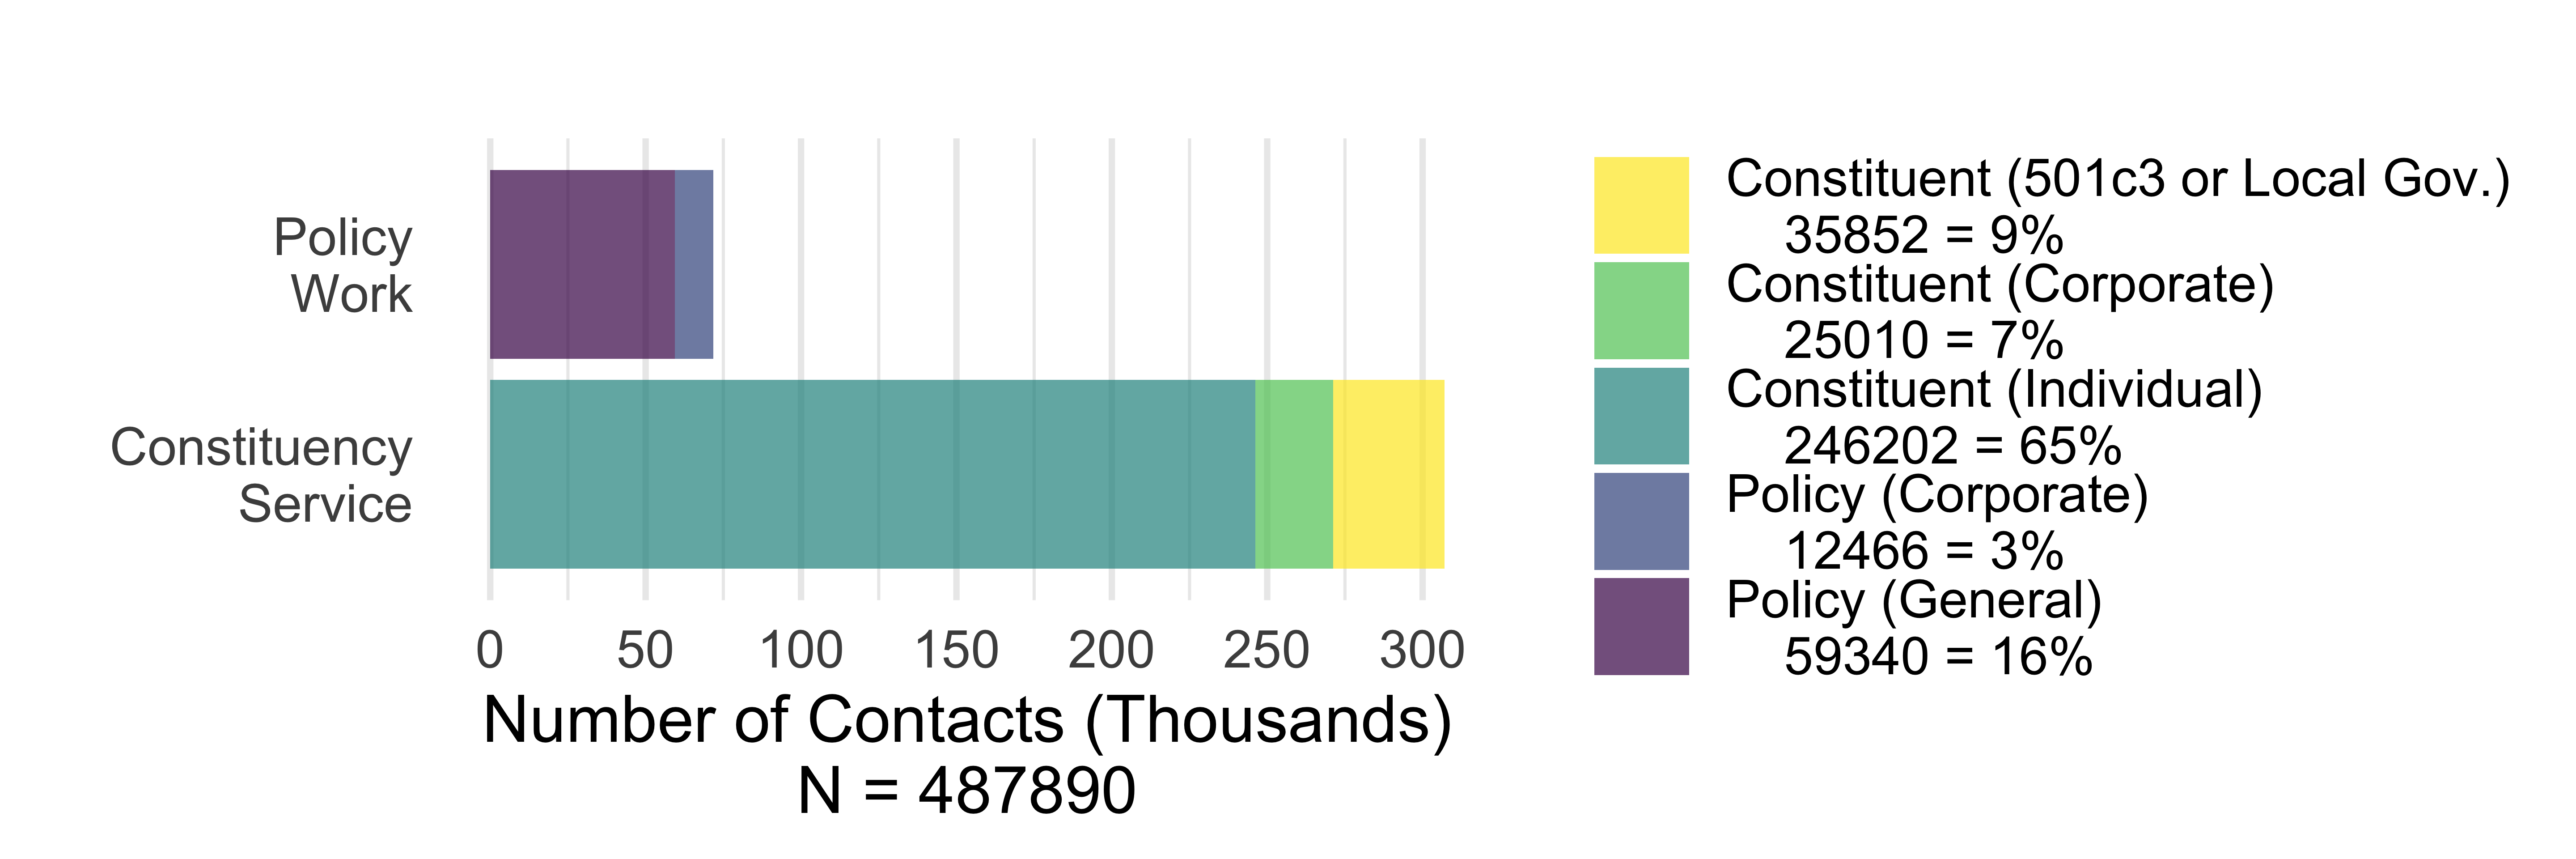
\includegraphics{figs/data_by_type-1}}
\end{figure}



To assess whether legislators shift their priorities as they gain experience and power, we further group requests into a broader ``constituency service"  category (including service for individuals, corporations, and nonprofits) and a broader ``policy work" category (including both general and industry-focused policy work). These two categories match those we go on to test in section \ref{s:prestige}. Using this more coarse classification, we find 82\% of contacts that chairs of committees make with federal agencies are focused on constituency service, and 87.9\% of contacts from members of prestige committees are focused on constituent service. Similarly, 89\% of the contacts legislators make in their first year are constituency service, and 87.5\% are constituency service in their sixth year. Descriptively, constituency service is the main reason for legislator's requests regardless of their position in Congress or tenure in Washington. 

\subsubsection{Levels of Contact with Federal Agencies are Highly Unequal}
Legislators vary significantly in how often they contact federal agencies. Gini coefficients for the number of contacts per year for the House and Senate are similar to those for income inequality in Mexico and the United States, respectively. Figure \ref{f:contact1} shows the average number of contact rates per year for House members (left-hand panel) and senators (right-hand panel). 
% DEVIN TODO REVISIONS BASED ON NEW FIGURES
In the Senate, Robert Byrd (D-WV) averaged 433 constituent service contacts per year. Other senators---such as Charles Schumer (D-NY) and John McCain (R-AZ)---have similarly high levels of contact with federal agencies. But other senators contact at a much lower rate. For example, John Kennedy (R-LA) made five constituency service requests during his first year in the Senate in 2017. On average, senators in our data set contact agencies 86 times per year.   
 
\begin{figure}
\centering
\caption{Variation in Average Legislator Requests by Percentile} \label{f:contact1} 
\begin{minipage}{\textwidth}
\scalebox{0.4}{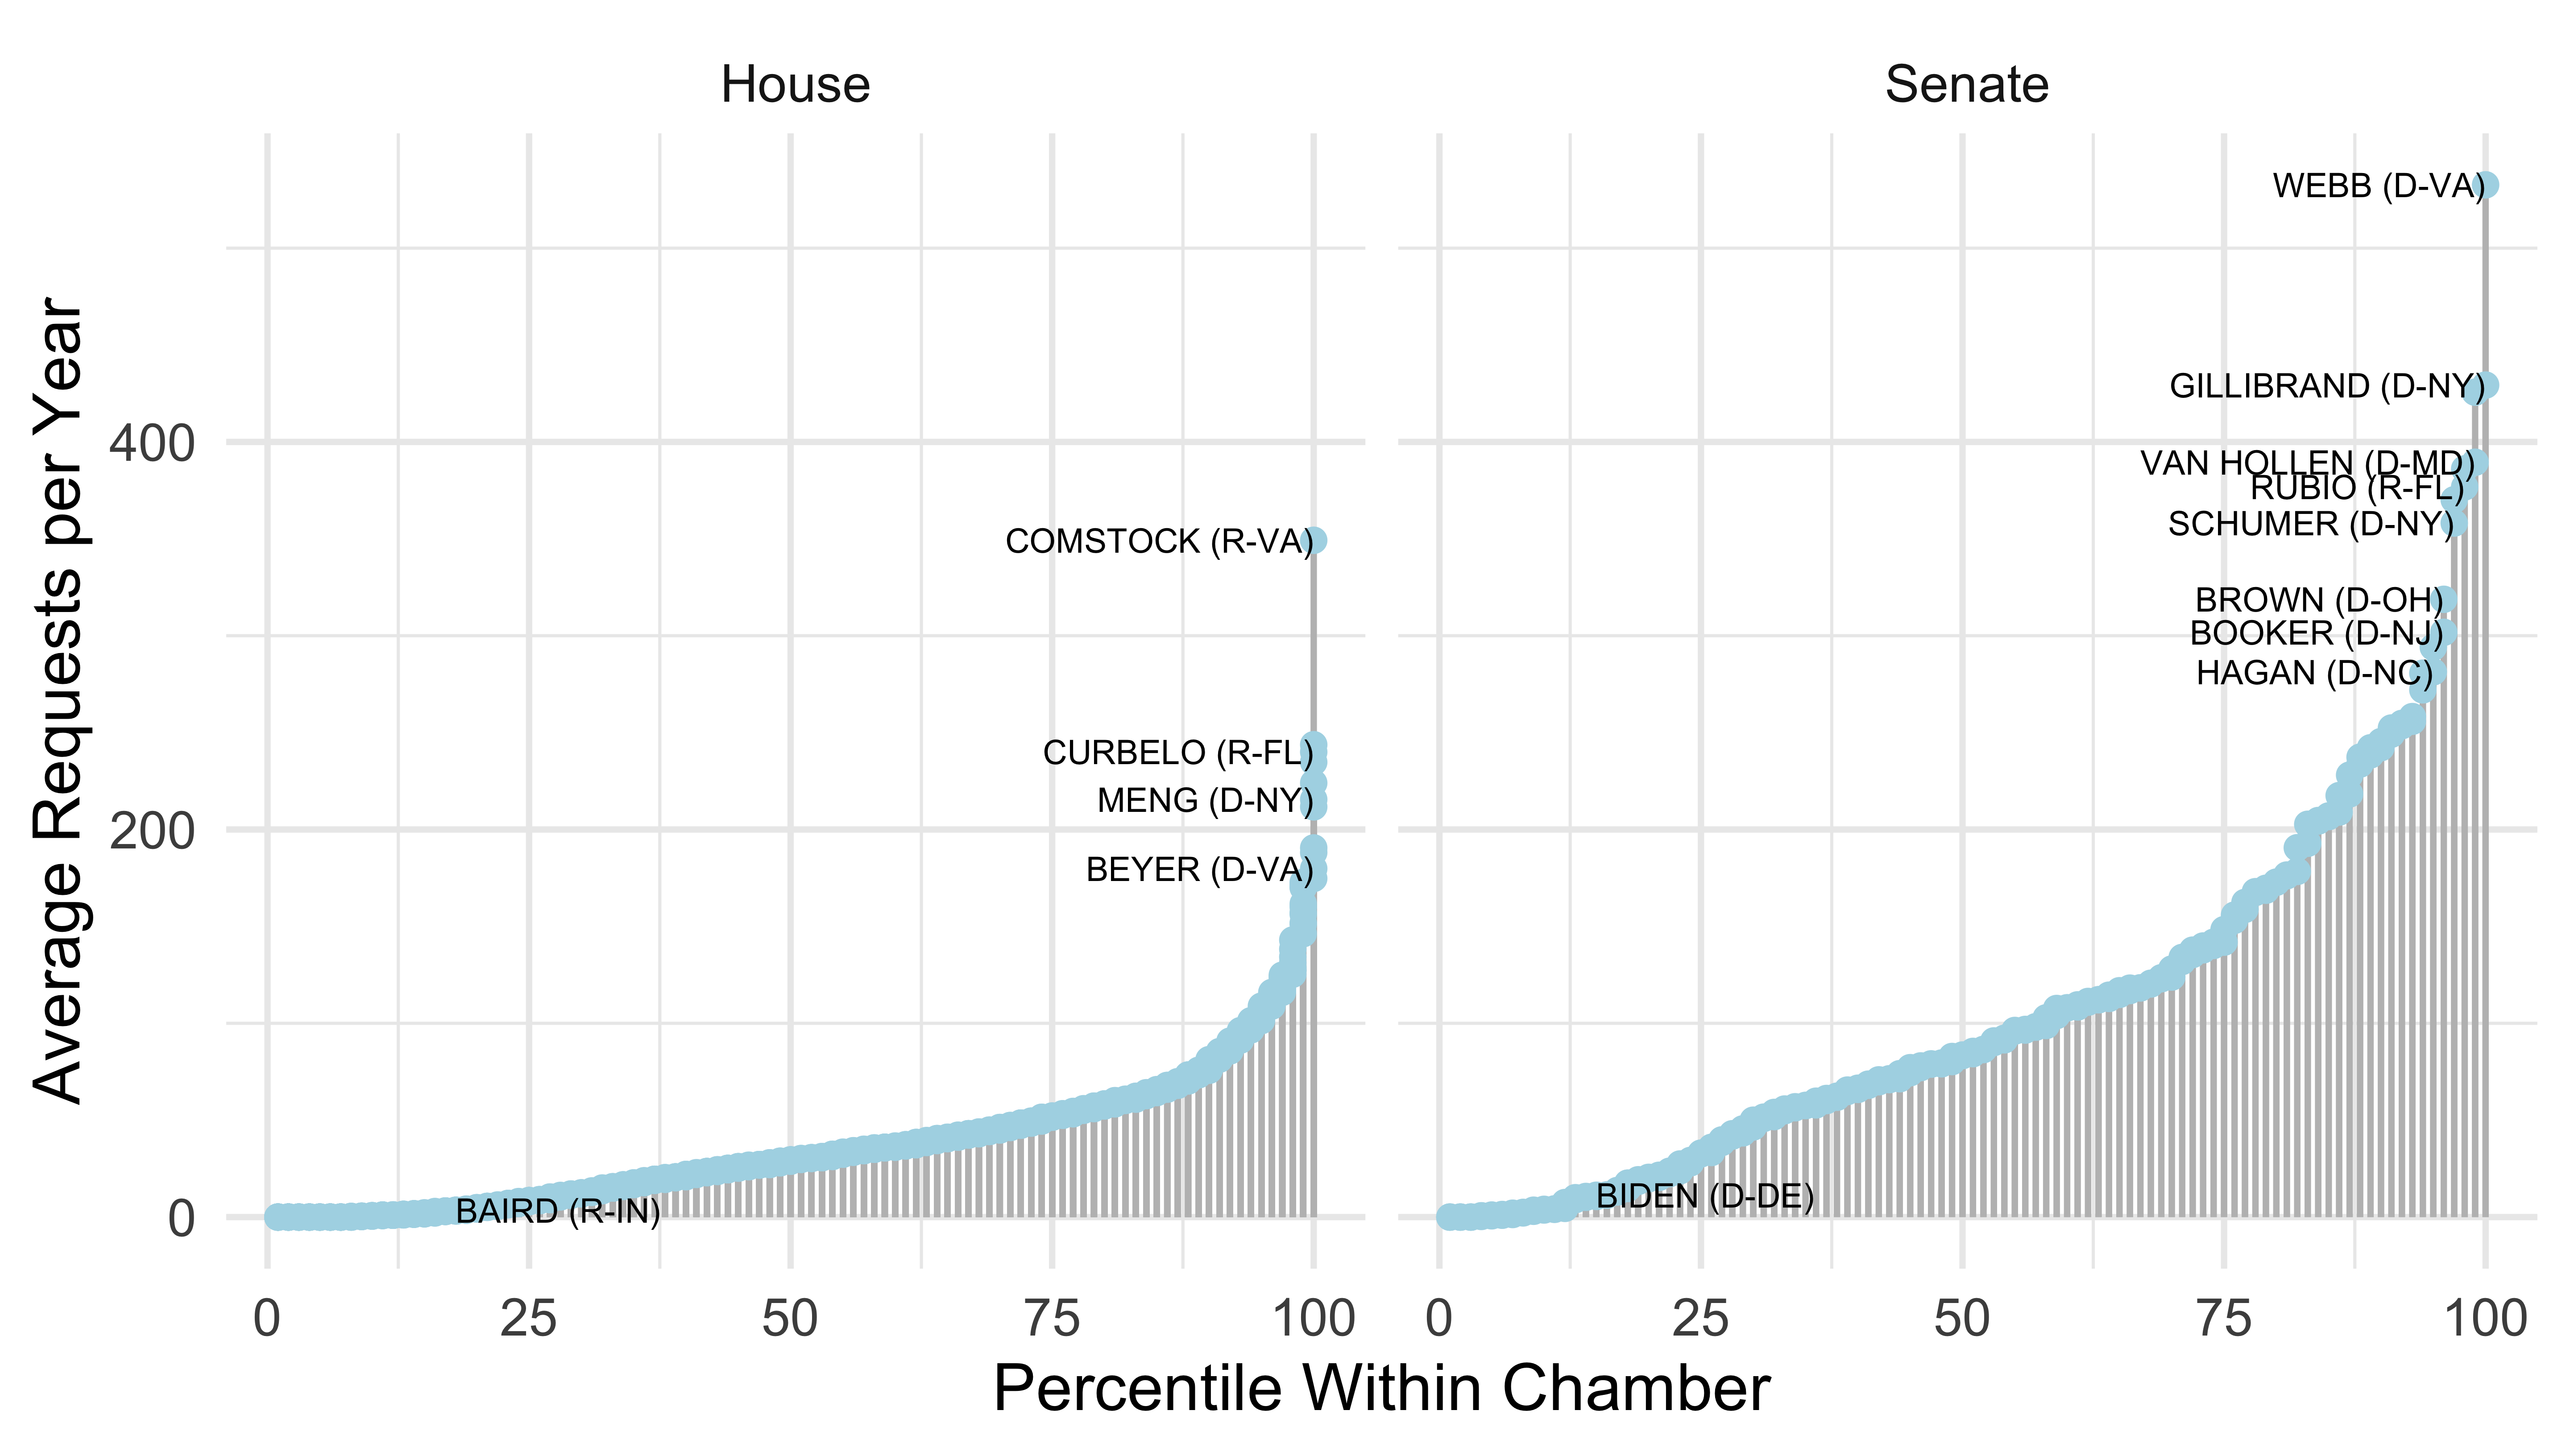
\includegraphics{figs/percentiles-1}}
\footnotetext{This figure presents the average number of contacts with federal agencies per year for House members (left-hand panel) and senators (right-hand panel), where the legislators' counts are sorted by their per year percentile rank. This reveals that senators and House members regularly contact federal agencies, but there is considerable variation in the level of contact across legislators.}
\end{minipage}
\end{figure}


We see similar variation in the House, but with lower overall levels of contact with federal agencies, reflecting lower resources and fewer constituents than senators. Frank Wolf (R-VA) averaged 306 contacts per year. Like the Senate, other legislators contacted at a much lower rate. Overall, House members averaged 29.4 contacts with federal agencies per year. But like the Senate, we large variability in the levels of contact across House members.  

Figure \ref{f:peryear} shows the number of requests per legislator over time, highlighting three Senators at the upper, middle, and lower parts of the distribution.

\begin{figure}
\centering
\caption{Variation in Legislator Requests by Year 2007-2017} \label{f:peryear} 
\begin{minipage}{\textwidth}
\scalebox{0.4}{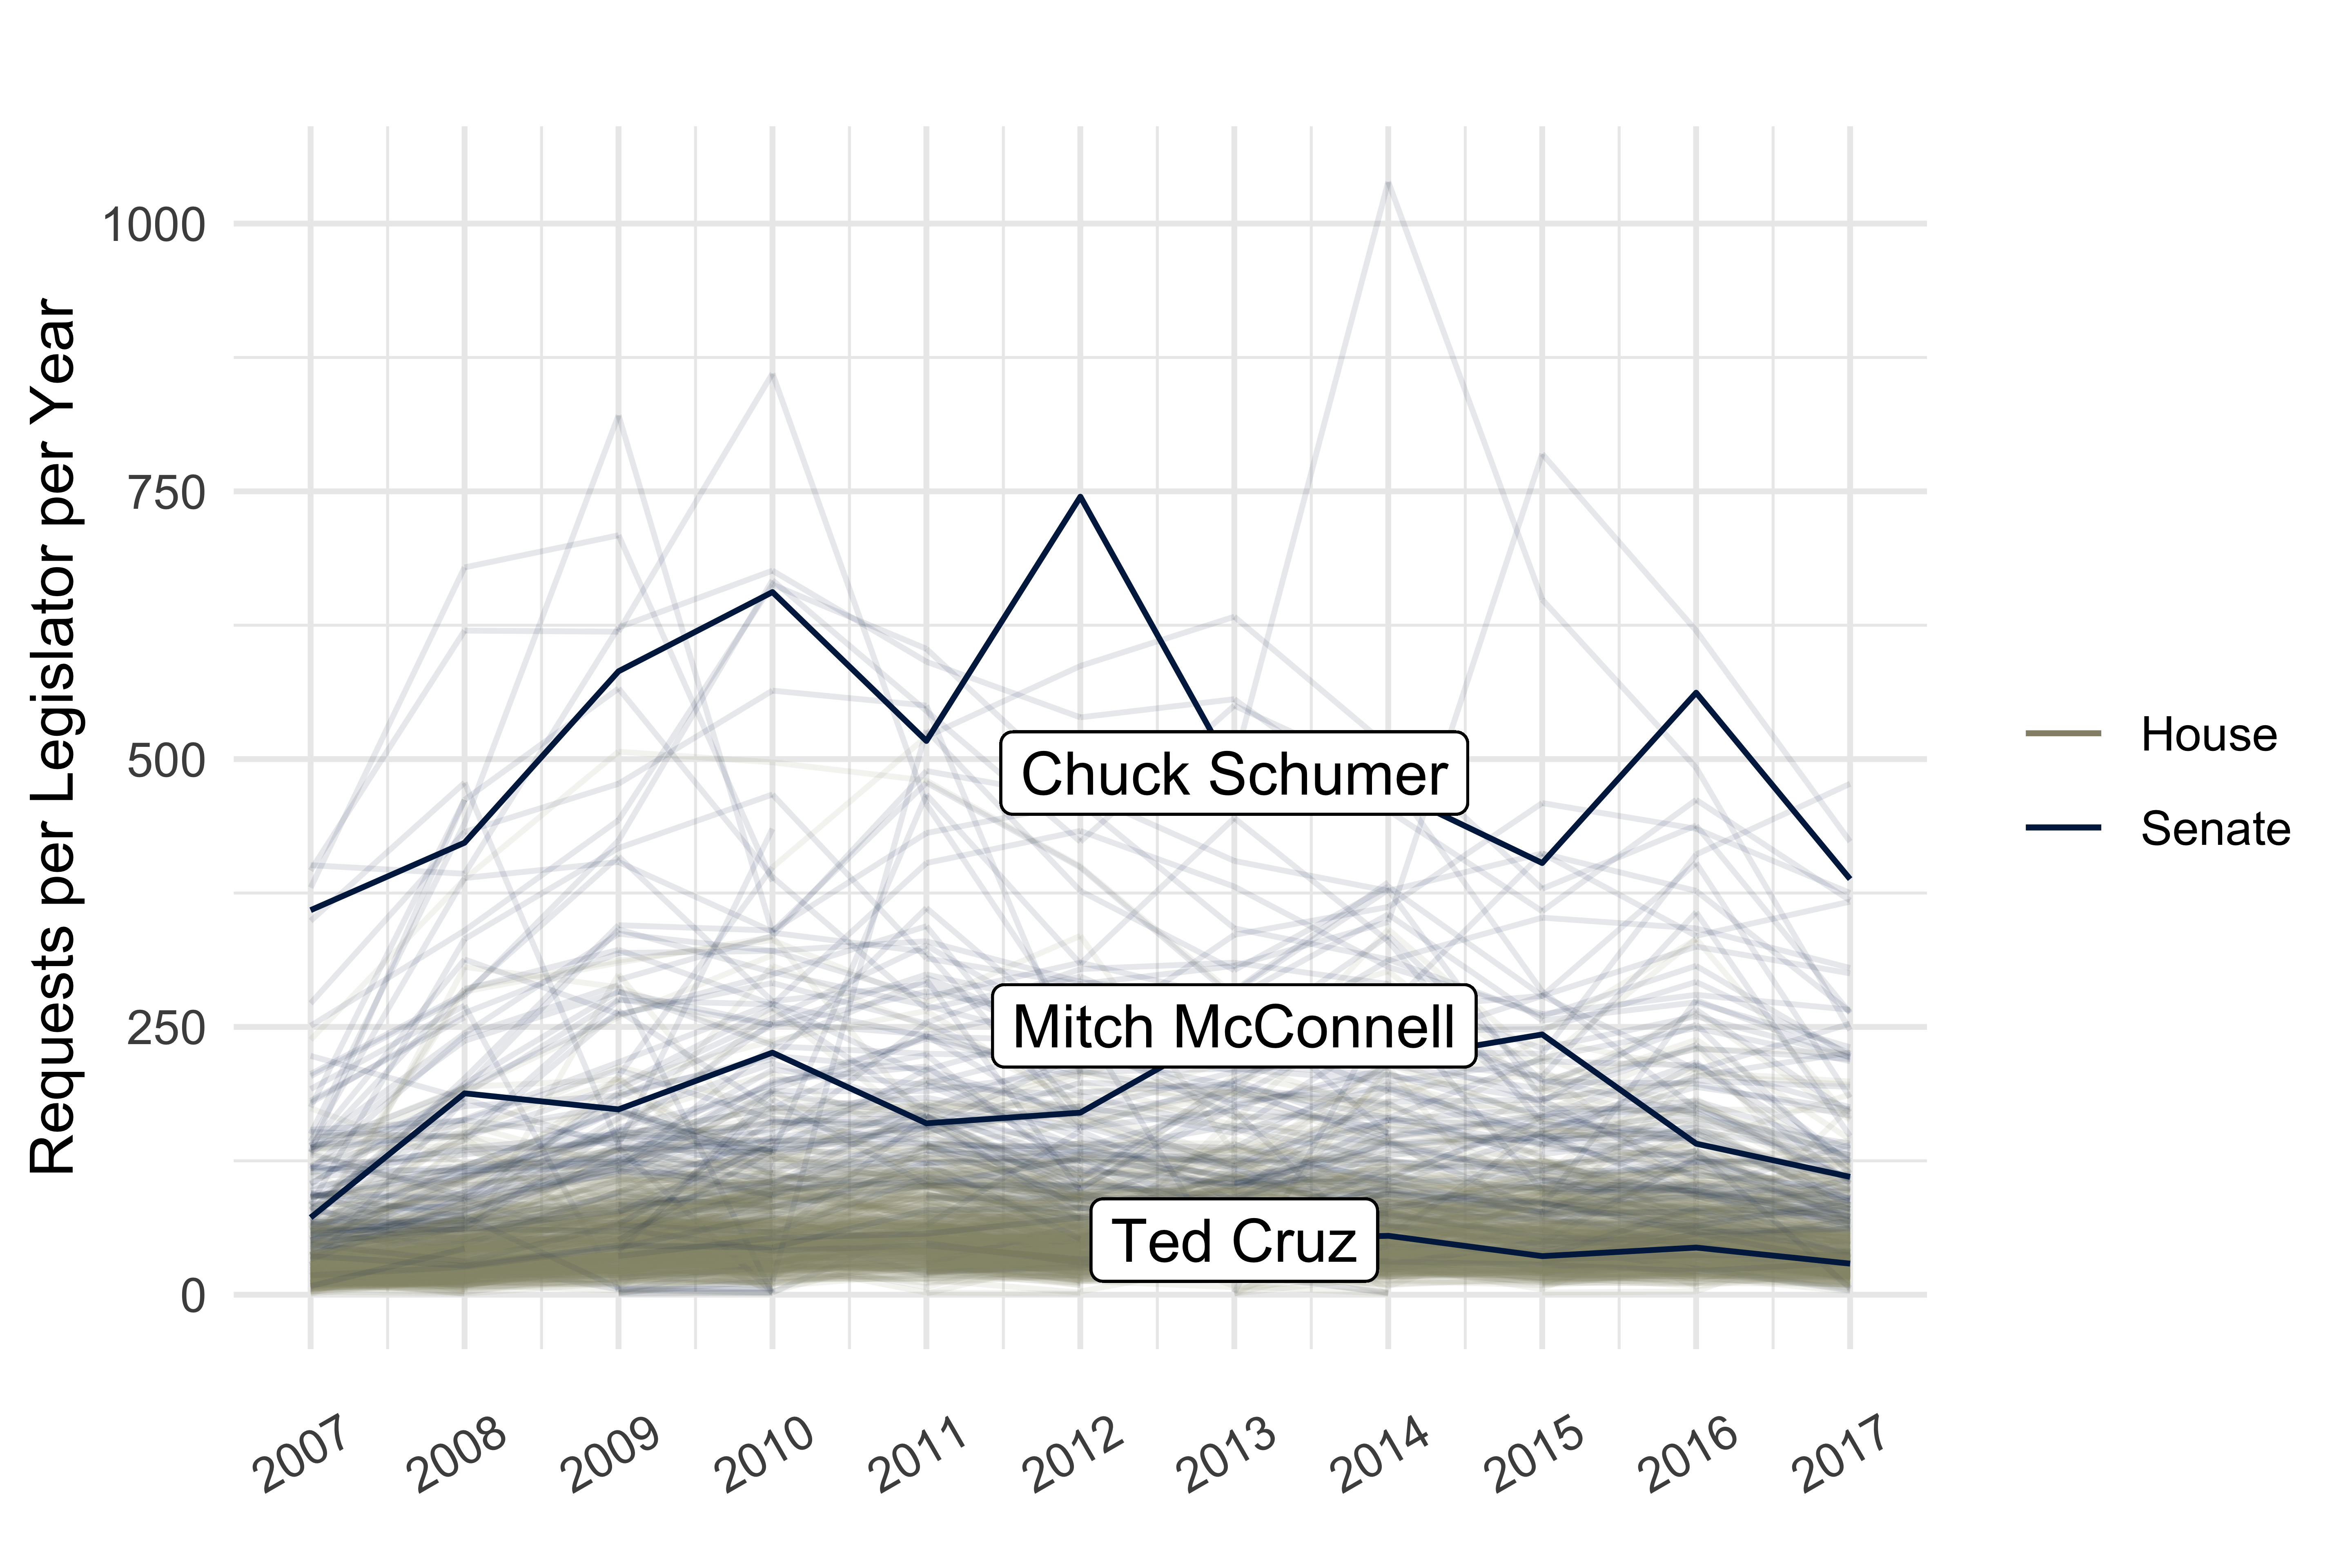
\includegraphics{figs/counts-per-year-1}}
\footnotetext{This figure presents the number of contacts with federal agencies per year for House members (left-hand panel) and senators (right-hand panel) over time. This reveals that senators and House considerable variation in the level of contact both within and across legislators.}
\end{minipage}
\end{figure}






\section{The Effect of Experience and Institutional Power}\label{s:results} 

Using this data set of requests to federal agencies, we now assess how legislators' changing position in Congress affects their provision of constituency service. First, we text theories rooted in legislator capacity by modeling the effects of institutional power on the overall \textit{level} of constituency service. Next, we test theories rooted in legislators' priorities by modeling the effects of institutional power on the overall \textit{ratio} of policy work to constituency service. Finally, we estimate the substantive impact of both increasing capacity and shifting priorities taken together. 

\subsection{The Effects of Experience and Institutional Power on Levels of Constituency Service}\label{s:prestige}

 Our primary models are a series of difference-in-differences regressions, similar to the specifications in \cite{BerryFowler2016}. Our most stringent specifications examine changes that are within legislator and agency.\footnote{We drop five member-congress level observations for congresses where the member switched political parties.} Specifically, we estimate regressions of the form: 

\begin{eqnarray}
Y_{ijt} & = & \boldsymbol{\beta}^{'} \textbf{Committee Position}_{it}  + \sum_{s = 1}^{6} \eta_{s} \text{I}\left(\text{tenure}_{it} = s\right) + \gamma_{ij} + \delta_{jt} + m_{it} + p_{it} + \epsilon_{ijt} \label{e:diff1}
\end{eqnarray}

Where $Y_{ijt}$ represents the number of requests legislator $i$ makes to agency $j$ in year $t$, so our analysis in this section focuses on the legislator-agency-year level. $\gamma_{ij}$ is a fixed effect for the legislator-agency pair. This fixed effect accounts for legislators' characteristics, such as legislators who are more skillful at filling constituency service requests than other legislators. Critically for our research design, this fixed effect also enables us to account for time-invariant constituent demand for constituency service with an agency, ensuring differences in constituent demand do not drive our results. It also accounts for characteristics such as the population of a state, its residents' demographic characteristics, and local industries that might be particularly likely to request help with specific agencies. This difference-in-difference design ensures that coefficients $\boldsymbol{\beta}$ capture variation related to changes in institutional power or experience, not other factors that may vary across districts, legislators, or agencies. The model also accounts for the different periods for which data were available from each agency. $\delta_{jt}$ is an agency-year fixed effect, takes into account agency-level common shocks across legislators in the provision of constituency service. 

Assuming that legislators' trends in the level of requests follow parallel paths, $\boldsymbol{\beta}$ represents the average effect of changing institutional power on a legislator's provision on constituency service. We focus on three measures of a legislator's committee position: (1) whether they are a committee chair, (2) whether they are a ranking member of a committee, and (3) whether they are members of a prestige committee. We focus on these committee positions because each represents a different way legislators can acquire more power while in Congress. As a legislator becomes a committee chair or ranking member, they have increased responsibilities when drafting and revising legislation. They also have increased access to committee resources to accomplish policy goals, particularly the power to direct committee staff. Similarly, legislators who join more prestigious committees gain the opportunity to shepherd policy through the legislative process.\footnote{We say that a House member is on a prestige committee if they are on Appropriations, Ways and Means, Rules, Budget, or Armed Services and if a senator is on Rules, Foreign Relations, Commerce, Budget, Armed Services, or Appropriations.} %CITE?

As \cite{BerryFowler2016} note, changes in legislators' committee assignments are often due to circumstances outside of the legislator's control, such as changing majority status, retirements on a committee, or exclusion due to losses from a previous election \citep{GrimmerPowell2013}. To violate the parallel trends assumptions, it would need to be the case that legislators differentially altered their rates of constituency service in anticipation of joining particular committees. To help avoid this violation, we include a series of controls that capture time-varying characteristics of a legislator that might confound our inference about the effect of committee prestige. Because legislators may make more requests to a president of the same party \citep{BerryBurdenHowell09}, it is a particular concern that legislators obtain new committee assignments when their party moves into or out of the majority or at the same time as the president party changes. To address these concerns, we include an indicator for whether the legislator's party is the majority in year $t$, $m_{it}$ and if the legislator of Congress is from the same party as the president in year $t$, $p_{it}$. Throughout, we cluster our standard errors at the legislator level.

In this same regression we also include indicators for legislators' first six years in Congress, $ \sum_{s = 1}^{6} \eta_{s} \text{tenure}_{it}$. The effects of interest $\eta_{1}, \eta_{2}, \hdots, \eta_{6}$ describe how a legislator's provision of constituency service at levels of seniority between one and six years differ from legislators who serve beyond six years. We focus on constituency service levels in each of the first six years of a legislator's tenure in Congress to assess how constituency service changes over their initial years in Congress. This design allows us to assess the extent to which new legislators face start-up costs. This specification, however, is ill-equipped to assess how electing a new representative affects the amount of constituency service a district receives. We address this in Section \ref{s:tenure_dist} by examining how electing a new representative affects the number of constituency service requests made on behalf of a district with a different difference-in-differences specification at the district-year level.   

%\subsection{The Effects of Experience and Institutional Power on the Level of Constituency Service} 

\begin{table}[hbt!]
\caption{The Effect Expierence and Institutional Power on Constituency Service} \label{t:prestige1}

\begin{minipage}{\textwidth}
\begin{center}
\begin{tabular}{l*{4}{c}}
\toprule
                    &\multicolumn{1}{c}{(1)}&\multicolumn{1}{c}{(2)}&\multicolumn{1}{c}{(3)}&\multicolumn{1}{c}{(4)}\\
\midrule
Committee Chair     &       0.712&       0.206&       0.209&      0.0366\\
                    &     (0.152)&    (0.0951)&    (0.0951)&    (0.0136)\\
Ranking Member      &       0.852&       0.123&       0.136&      0.0250\\
                    &     (0.156)&    (0.0967)&    (0.0970)&    (0.0119)\\
Prestige Committee  &       0.470&      0.0790&      0.0746&      0.0210\\
                    &    (0.0665)&    (0.0508)&    (0.0519)&    (0.0103)\\
First Year          &      -0.255&      -0.139&      -0.144&     -0.0124\\
                    &    (0.0519)&    (0.0489)&    (0.0473)&   (0.00979)\\
Second Year         &     -0.0713&      0.0177&      0.0248&      0.0239\\
                    &    (0.0585)&    (0.0474)&    (0.0469)&   (0.00908)\\
Third Year          &     -0.0198&      0.0764&      0.0595&      0.0338\\
                    &    (0.0625)&    (0.0450)&    (0.0444)&   (0.00823)\\
Fourth Year         &     0.00126&      0.0707&      0.0522&      0.0260\\
                    &    (0.0664)&    (0.0455)&    (0.0431)&   (0.00806)\\
Fifth Year          &     -0.0515&      0.0280&      0.0266&      0.0164\\
                    &    (0.0611)&    (0.0377)&    (0.0367)&   (0.00701)\\
Sixth Year          &     -0.0156&      0.0504&      0.0744&    0.000378\\
                    &    (0.0728)&    (0.0536)&    (0.0516)&   (0.00762)\\
\midrule
Majority, President's Party&  \checkmark&  \checkmark&  \checkmark&  \checkmark\\
Legislator $\times$ Agency Fixed Effects&            &  \checkmark&  \checkmark&  \checkmark\\
Year $\times$ Agency Fixed Effects&            &  \checkmark&  \checkmark&  \checkmark\\
All Legislators     &  \checkmark&  \checkmark&            &  \checkmark\\
Serve At Least Second Term&            &            &  \checkmark&            \\
Dependent Variable  &       Count&       Count&       Count&Log(Count + 1)\\
Observations        &      412111&      412111&      388997&      412111\\
\bottomrule
\multicolumn{5}{l}{\footnotesize Robust standard errors in parentheses, clustered at legislator level}\\
\end{tabular}

\end{center}
\footnotetext{Column 1 shows the average differences across committee assignments and years in Congress. Column 2 presents the difference-in-differences estimates. Column 3 subsets to legislators who serve at least 3 years in Congress. Column 4 takes the Log of the counts + 1 as the dependent variable.}
\end{minipage}
\end{table}

Table \ref{t:prestige1} provides the coefficient estimates from Equation \ref{e:diff1}. We focus first on the estimated effect of increased committee prestige. Table \ref{t:prestige1} shows that as legislators acquire more prestige, their rates of constituency service increase. All coefficients represent the average additional requests per year \textit{per agency}; per legislator per year effects are simply these coefficients times 83.  Model 1 (the first column of Table \ref{t:prestige1}) shows that this is true in a cross-sectional comparison across legislators. Model 1 excludes the legislator-agency and year-agency fixed effects, but it does include controls for majority status and being from the same party as the president. 

\subsubsection{The Effect of Institutional Power on Levels of Constituency Service}\label{s:prestigeresults} 

Table 1 shows that committee chairs, ranking members, members of prestige committees, and members of the oversight committee provide substantially more constituency service than other legislators. These cross-sectional differences, however, conflate a legislator's institutional position with other legislator characteristics. If legislators who are better at their jobs or who exert more effort are also selected for more prestigious committee positions, then the estimates from Model 1 confound legislators' overall ability with their institutional position.   




To address potential confounding in across-legislator comparisons, the estimates from Model 2 (Column 2 of Table \ref{t:prestige1}) provide the estimated effects from the difference-in-differences specification in Equation \ref{e:diff1}. Across all measures of institutional power, we find that more power increases the level of constituency service that legislators provide. Consider first the effect of being a committee chair. We estimate that becoming a committee chair causes an increase of 0.206 constituency service requests \textit{per agency} (95-percent confidence interval [0.02, 0.39]). Across all agencies, this represents an increase of approximately 13.6 additional constituency service requests per year, 20\% of the average number of requests per year in our data. There is a smaller increase for individuals who become ranking members and those who join a Prestige Committee, though the increase is statistically significant for the prestige committee. Becoming a ranking member of a committee causes an increase of 0.123 contacts per agency while joining a prestige committee causes a 0.079 per agency increase in the number of constituency service contacts a member of Congress makes.

The findings in Table \ref{t:prestige1} are robust to alternative specifications and measures of the dependent variable. For example, we might be concerned that legislators with exceptionally high constituency service levels drive the results. The fourth column shows that we obtain the same findings if we use $\log (Y_{ijt} + 1)$ in our difference-in-differences specification. Further, our results are not due to differential attrition. The third column shows that we obtain nearly identical results if we restrict our analysis to legislators who serve beyond three years.    

This section has shown that acquiring power in Washington causes legislators to increase constituency service levels. This increase occurs across all three measures of committee position that we examine but is most robust for committee chairs. 


\subsubsection{The Effect of Legislator Experience on Levels of Constituency Service}\label{s:tenure} 

As legislators acquire more power in Washington, we find that they increase their provision of constituency service. While this suggests that more powerful legislators are paying more attention to their constituents, it could still be the case that as legislators gain experience in Washington, they decrease their constituency service provision. To test whether this is the case, we use the estimates in Table \ref{t:prestige1} but now focus on the coefficients in legislators' first six years in office. The reference group is representatives who have served longer than six years.\footnote{Interpreting these coefficients requires that we assume the effects of tenure and committee assignment are linearly separable. This assumption is reasonable because most legislators do not become chairs, ranking members, join prestige committees in their first six years in Congress, almost none in their first two years.} 


The first column of Table \ref{t:prestige1} shows that there are large cross-sectional differences: legislators in their first year make many fewer contacts than more experienced legislators, with first-year legislators making approximately 0.255 fewer requests per agency than legislators in their seventh year or beyond. This difference shrinks in the second year and then is mostly gone. But we advise caution in interpreting the differences in Column 1 because they conflate the effect of increased experience in Congress with other characteristics that may correlate with whether a legislator remains in office and thus whether we observe them in later years.   


% To test this hypothesis, we use a similar empirical approach in the previous section but now focus on the first years of an individual's service in Washington. Specifically, we estimate a difference-in-differences regression of the form: 

% \begin{eqnarray}
% Y_{ijt} & = & \sum_{s=1}^{6} \beta_{s} \text{tenure}_{s[it]} + \gamma_{ij} + \delta_{t} + m_{it} + p_{it} + \epsilon_{ijt} \label{e:diff2}
% \end{eqnarray} 

% where we include fixed effects for each legislator-agency pair ($\gamma_{ij}$), a time fixed effect ($\delta_{t}$), and indicators for a legislator's status in the majority ($m_{it}$) or in the president's party ($p_{it}$).  


%We are interested in both the size of these coefficients--which inform how legislators' provision of constituency service compares to legislators who have remained in office longer than seven years---and comparisons across the coefficients---which describe how the provision of constituency service changes over the first six years in office. Our comparisons across these first years do not depend on how many years we include in the analysis. But the ``reference" category can lead to slightly different conclusions about the level of service that new legislators provide compared to more experienced members. This section focuses on these first years because this is the time frame for many term limit proposals. Further, this is the range where we have the best evidence for the year-to-year shifts in how legislators provide service. The restriction in Equation \ref{e:diff2} is not consequential for the conclusions that we reach. We show in Appendix ZZ that the main patterns that we uncover are consistent regardless of how many years we include in our analysis. And as we show in section YY, we find similar patterns when examining what occurs after a new legislator takes office. 

%The first column of Table \ref{t:tenure1} is a cross-sectional regression that compares the provision of constituency service across legislators' first six years in Congress, while also including indicator's for a legislator's majority party status and whether they are members of the president's party. This regression shows that new legislators provide substantially lower levels of constituency service than their colleagues in their second year of service in Congress: legislators in their first year make about 0.135 fewer constituency service requests per agency than legislators in their second year and 0.2 fewer requests than legislators in their third year. Across all six years, we find that newer legislators are, on average, making fewer contacts with federal agencies than their more experienced colleagues.  


% \begin{table}[hbt!]
% \caption{Estimating Effect of Tenure on Constituency Service Provision} \label{t:tenure1}
% \begin{minipage} {\textwidth}
% \begin{center}
% \begin{tabular}{l*{4}{c}}
\toprule
                    &\multicolumn{1}{c}{(1)}&\multicolumn{1}{c}{(2)}&\multicolumn{1}{c}{(3)}&\multicolumn{1}{c}{(4)}\\
\midrule
First Year          &      -0.478&      -0.179&      -0.183&     -0.0317\\
                    &    (0.0349)&    (0.0347)&    (0.0351)&   (0.00527)\\
Second Year         &      -0.344&     -0.0665&     -0.0630&   -0.000440\\
                    &    (0.0375)&    (0.0335)&    (0.0337)&   (0.00510)\\
Third Year          &      -0.274&    -0.00694&    -0.00697&     0.00662\\
                    &    (0.0376)&    (0.0328)&    (0.0328)&   (0.00482)\\
Fourth Year         &      -0.237&      0.0200&      0.0200&      0.0126\\
                    &    (0.0409)&    (0.0310)&    (0.0310)&   (0.00470)\\
Fifth Year          &      -0.238&    0.000539&    0.000506&   -0.000442\\
                    &    (0.0388)&    (0.0296)&    (0.0296)&   (0.00434)\\
Sixth Year          &      -0.220&      0.0204&      0.0204&     0.00242\\
                    &    (0.0401)&    (0.0278)&    (0.0278)&   (0.00414)\\
\midrule
Majority, President's Party&  \checkmark&  \checkmark&  \checkmark&  \checkmark\\
Legislator $\times$ Agency Fixed Effects&            &  \checkmark&  \checkmark&  \checkmark\\
Year Fixed Effects  &            &  \checkmark&  \checkmark&  \checkmark\\
All Legislators     &  \checkmark&  \checkmark&            &  \checkmark\\
Serve At Least Second Term&            &            &  \checkmark&            \\
Dependent Variable  &       Count&       Count&       Count&Log(Count + 1)\\
Observations        &      337610&      337610&      330215&      337610\\
\bottomrule
\multicolumn{5}{l}{\footnotesize Robust standard errors in parentheses, clustered at legislator x agency level}\\
\end{tabular}

% \end{center}
% \footnotetext{This table shows. Model 1: no fixed effects. Model 2: legislator x agency and year model 3: only those legislators who survive their first election. }
% \end{minipage}
% \end{table}


To account for possible differences in legislators who obtain different levels of tenure, the second column of Table \ref{t:prestige1} estimates the difference-in-differences specification in Equation \ref{e:diff1}. The tenure coefficients show that legislators provide less constituency service in their first year in office. As they acquire experience in Congress, they make more requests to federal agencies. In their first year in office, legislators provide 0.16 fewer requests per agency than legislators in their second year and 0.215 fewer requests than legislators in their third year--both differences are statistically significant at conventional levels. The overall increase in levels of constituency service from a legislator's first to third year is similar in size to the increase that comes from becoming a member of the oversight committee: resulting in about 14.6 more constituency service requests per year. Once legislators enter their fourth year, their behavior no longer differs from more experienced legislators. We find small and statistically insignificant differences for legislators in their fourth through sixth years. As legislators acquire experience and build their office's organizational capacity in their first two years, they make more contacts with federal agencies.  

As with the analysis of committee prestige, the findings in Table \ref{t:prestige1} are robust to alternative specifications. Despite the difference-in-difference design, we might still be concerned that the set of legislators who serve in their third year are different than the legislators who serve in the first years. If this were the case, then our findings would be the result of both the experience and a selection effect due to House members who win reelection, a potential indication that they are better able to perform the job than other legislators. To address the potentially different samples in each year, the third column of Table \ref{t:prestige1} assesses the changes in the number of contacts of federal agencies for legislators who serve in Congress for at least three years. The pattern is similar: legislators initially providing less constituency service in their first two years than they do in subsequent years. And Column 4 in Table \ref{t:prestige1} shows that the results are robust to analyzing $\log(Y_{ijt} + 1)$, ensuring that our results are not because of outliers.  

\subsubsection{The Effect of Electing a New Representative on the Level of Constituency Service}\label{s:tenure_dist}

In the previous section, we showed that legislators make fewer requests to federal agencies in their first year in office but that the number of requests stabilizes after their third year. We now turn to a related question: how does the level of constituency service to a district change after the election of a new representative? Rather than examining changes in the number of requests by making within-legislator comparisons, we now make within-district comparisons to assess how electing a new legislator affects the total number of requests a district's representative makes. In other words, within-district comparisons enable us to assess the costs or benefits of electing a new representative compared to an incumbent.


To make this comparison, we change the level of our analysis and focus now on the number of contacts made from the representative of a particular state or district $i$ in a year $t$, $Y_{it}$. We again use a difference-in-differences approach to account for district-specific characteristics and over-time changes in how legislators provide constituency service. Specifically, we estimate regressions of the form: 


\begin{eqnarray}
Y_{it} & = & \beta_{1}\text{New Member}_{it} + \sum_{s = 2}^{6} \beta_{s} \text{tenure}_{s[it]} + \gamma_{i} + \delta_{t} + \epsilon_{it} \label{e:district1} 
\end{eqnarray}

Where $\gamma_{i}$ is a district-specific fixed effect that accounts for each district's particular demographic characteristics, along with the levels of demand from district residents. $\delta_{t}$ is a year fixed effect that takes into account common shocks. Our key result of interest, $\beta_{1}$, is the effect of a district electing a new representative. To understand how the effect of a new representative changes over time, we estimate district-level differences for a legislator's second ($\beta_{2}$) through sixth-year ($\beta_{6})$.\footnote{It is worth noting that this treatment is fundamentally different for a district than within-legislator variation. In each election, each district either allows their incumbent to acquire another term or replaces her. This is different from within-legislator comparisons because legislators can only acquire more tenure or leave the chamber. A within-legislator analysis estimates the service provided by incumbents with more or less experience; it cannot estimate the impact of the choice of an incumbent or a new representative incumbent.} % TODO THIS FOOTNOTE IS REPETITIVE.

The first column of Table \ref{t:district2} provides a simple difference-in-means for districts represented by a new member and then for legislators in their first six years in office. Comparing across districts, districts represented by new legislators receive substantially lower levels of constituency service. On average, districts with a new representative have 35.2 fewer constituency service requests made on their behalf. The magnitude of this difference shrinks for districts represented by legislators in their second year (23.75 fewer constituency service requests). It then reaches a relatively stable number for districts represented by legislators in their third through sixth years.%, with some slight evidence that legislators make more contacts in election years---the even-numbered years of tenure for the vast majority of legislators in our sample. 



\begin{table}[hbt!]
\caption{The Effect of Electing New Members on a District's Level of Constituency Service} \label{t:district2}
\begin{minipage}{\textwidth}
\begin{center}
\begin{tabular}{l*{4}{c}}
\toprule
                    &\multicolumn{1}{c}{(1)}&\multicolumn{1}{c}{(2)}&\multicolumn{1}{c}{(3)}&\multicolumn{1}{c}{(4)}\\
\midrule
New Legislator      &      -35.23&      -35.55&      -14.89&      -123.5\\
                    &     (4.445)&     (4.500)&     (2.627)&     (13.84)\\
Legislator 2nd Year &      -23.75&      -20.31&      -4.402&      -79.99\\
                    &     (4.464)&     (3.949)&     (2.662)&     (11.34)\\
Legislator 3rd Year &      -13.08&      -13.53&      -1.630&      -49.48\\
                    &     (4.886)&     (4.448)&     (2.586)&     (16.07)\\
Legislator 4th Year &      -12.43&      -9.077&       0.268&      -26.92\\
                    &     (5.216)&     (4.276)&     (2.736)&     (16.30)\\
Legislator 5th Year &      -14.92&      -11.58&      -3.810&      -31.58\\
                    &     (4.416)&     (3.591)&     (2.128)&     (13.11)\\
Legislator 6th Year &      -13.56&      -5.216&      -1.638&      -2.500\\
                    &     (5.104)&     (3.790)&     (2.239)&     (14.46)\\
\midrule
District Fixed Effects&            &  \checkmark&  \checkmark&  \checkmark\\
Year Fixed Effects  &            &  \checkmark&  \checkmark&  \checkmark\\
All Districts       &  \checkmark&  \checkmark&            &            \\
House Only          &            &            &  \checkmark&            \\
Senate Only         &            &            &            &  \checkmark\\
Observations        &        6578&        6578&        5338&        1240\\
\bottomrule
\multicolumn{5}{l}{\footnotesize Robust standard errors in parentheses, clustered at district level}\\
\end{tabular}

\end{center}
\footnotetext{This table shows how constituent service at the district level changes over time. Model 1 is a cross sectional comparison excluding district and year fixed effects. The second column is a district x year difference in differences model. Column 3 focuses the diff-in-diff on legislators who survive their first election. }
\end{minipage}
\end{table}


To account for differences in district size, demographics, and demand for constituency service, the second column of Table \ref{t:district2} estimates the difference-in-differences from Equation \ref{e:district1}. In this specification, we see a large causal effect of a new member taking over: electing a new member causes a decrease of 36 constituency service requests (95-percent confidence interval [-44, -27]), a sizable change in the number of service requests representatives make on behalf of their new constituents. %TODO PERCENT CHANGE 
The effect of electing a new representative, however, dissipates quickly. Districts represented by a legislator in her second year of service receive 12 fewer constituency service requests---still a substantively significant decrease in contact with federal agencies, but not as drastic as the first year decrease. After the second year, the differences are smaller in magnitude. This phenomenon--new legislators providing substantially fewer requests--persists when examining the House (Column 3) and the Senate (Column 4) separately. In short, new legislators make fewer contacts for their constituents than well-established elected officials.  


\paragraph{The Costs of Newly Elected Members} Taken together, our results demonstrate that new legislators provide much less constituency service. Legislators in their first year provide much less constituency service than they do in their second year and reach a stable level of service in their third year. Further, when districts elect a new representative or senator, they experience a sharp decrease in constituency service requests made on their behalf. Rather than experienced legislators forgetting about their districts, our evidence suggests that newly elected legislators experience substantial start-up costs and struggle to provide the levels of service that experienced legislators deliver to their constituents.  


\subsection{The Effect of Experience and Institutional Power on Legislators' Priorities}\label{s:priority} 
To assess legislators' ratio of policy work to constituency service, we use the hand-coded data described in Section \ref{s:data}. The dependent variable in Table \ref{t:priority} is the number of policy requests divided by the number of constituency service requests per legislator per year. These models test whether legislators' priorities shift among goals as they gain experience and power in Congress.

\begin{table}
\begin{center}
\begin{minipage}{\textwidth}
\caption{The Effect of Expierence and Institutional Power on the Ratio of Policy Work to Constituency Service} \label{t:priority}
\centering
\begin{tabular}{l*{2}{c}}
\toprule
                    &\multicolumn{1}{c}{(1)}&\multicolumn{1}{c}{(2)}\\
\midrule
Prestige            &      0.0220&     -0.0105\\
                    &   (0.00777)&    (0.0101)\\
Chair               &     -0.0744&     -0.0875\\
                    &    (0.0157)&    (0.0175)\\
Ranking Minority    &    0.000387&     -0.0346\\
                    &    (0.0138)&    (0.0142)\\
First Year          &      0.0428&      0.0223\\
                    &   (0.00918)&    (0.0115)\\
Second Year         &      0.0744&      0.0546\\
                    &   (0.00888)&    (0.0111)\\
Third Year          &      0.0400&      0.0235\\
                    &   (0.00888)&    (0.0107)\\
Fourth Year         &      0.0357&      0.0192\\
                    &   (0.00970)&    (0.0108)\\
Fifth Year          &     0.00801&    -0.00254\\
                    &   (0.00994)&    (0.0105)\\
Sixth Year          &      0.0533&      0.0431\\
                    &   (0.00933)&   (0.00940)\\
\midrule
Majority            &            &  \checkmark\\
Legislator Fixed Effects&            &  \checkmark\\
Year Fixed Effects  &            &  \checkmark\\
Observations        &        6442&        6442\\
\bottomrule
\multicolumn{3}{l}{\footnotesize Robust standard errors in parentheses, clustered at legislator level}\\
\end{tabular}

\footnotetext{This table shows how the proportion of contacts focused on constituency service changes as legislators acquire more expiernece and power in Congress.}
\end{minipage}
\end{center}
\end{table}


Table \ref{t:priority} shows that legislators increase the ratio of policy work to constituency service as they obtain more experience and prestigious committee assignments in Congress. The first column of Table \ref{t:priority} shows how the proportion of policy work to constituency service differs \textit{across} legislators' in their first six years in office and for legislators who acquire committee positions. We find that a higher proportion of legislators' contacts are focused on constituency service in their initial years in office.
% IS THIS TRUE? NO.
While the ratio of policy work to constituency service is conditional on the levels of each, the inference we wish to make about the ratio does not depend on these levels; we are not using the ratio to infer the level (e.g. that a lower share of constituency service means a lower level). Instead, the theory of prioritization is directly about the ratio, regardless of the level. Levels may interact with the ratio, but not in ways that do not mean the same thing for our theory: that legislators are prioritizing one thing over the other. 

%Our research design cannot identify the effect of increased tenure on the ratio of policy work to constituency service because to make the assessment implicitly requires conditioning on a post-treatment variable: contacting federal agencies. Nonetheless, a difference-in-differences regression can provide interesting descriptive evidence about how the content of legislators' contact with federal agencies changes as they gain more experience. To that end, 
Column 2 uses a difference-in-differences regression to assess how tenure in Washington affects the proportion of contacts focused on constituency service. 
% TODO DESCRIBE TABLE 2, MODEL 2 HERE 


%\subsection{The Joint Effect of Changing Power and Priorities on Levels of Constituency Service}\label{s:joint} 

%In Section \ref{s:descriptive}, we showed that the vast majority of contacts with federal agencies focus on constituency service. In Section \ref{s:presitge} we showed that legislators provide more constituency service as they gain experience. In section \ref{s:priorty} we showed that legislators also increase their ratio of policy work to constituency service when they gain experience and power. These latter two findings have potentially conflicting effects on the overall level of constituency service (accounting for both shifts in capacity and priority). Thus, we now turn to the net effect on levels of constituency service, accounting for the effects of both increasing capacity on the level of constituency service (Table \ref{t:capacity}) shifting priorities on the ratio of policy work to constituency service (Table \ref{t:priority}




%Shifting priorities--the change in the ratio of policy work to constituency service--do not overpower the effects of increased capacity and power--the change in the overall number of requests to federal agencies, with even more powerful legislators focused primarily on constituency service. 

%The next section investigates an alternative explanation for our findings: shifts in demand for constituency service. We show that demand matters, but not in ways that undermine the above conclusions.


\section{The Effects of Demand for Constituency Service}\label{s:demand} 

This section shows that demand for constituency service affects the level of constituency service that members provide. However, it does not appear that demand-side shifts can explain the specific within-legislator or within-district variation we observe with changing committee assignments and increased tenure. First, we show that constituent demand does drive legislators' constituency service requests to the agencies best suited to address the district's needs. Then, we show that this demand does not shift within or across legislators in ways that we would expect to see if shifting constituent demand explained the within-legislator and within-district variation in constituency service discussed in section \ref{s:prestigeresults}.

\subsection{District Characteristics Affect the Provision of Constituency Service }

The characteristics of their districts help inform which agencies that legislators contact. We find that population size correlates with the overall number of requests and that constituency characteristics--the proportion of veterans and the proportion over 65--correlate with the distribution of requests across agencies. These correlations provide face-validity for our measures of representation, but they also suggest that cross-sectional comparisons may conflate legislator choices with characteristics of districts. Given this potential conflation, our models below include fixed effects for each legislator-agency pair, leveraging within-district and within-agency variation.  

We expect senators who represent larger states to make more requests. Senators from larger states have a larger number of constituents to serve, and they receive a larger budget to handle that increase in requests.
Figure \ref{f:stateSize} shows that this is the case: senators from larger states provide more constituency service on average. Senators from larger states, like John Cornyn (R-TX), Barbara Boxer (D-CA), and Pat Toomey (R-PA), average more requests per year than legislators from smaller states. While the number of legislator requests is associated with population size, Figure \ref{f:stateSize} also shows significant variation in the level of service that senators provide, even among states of similar sizes.  

\begin{figure}
\centering
\caption{Average Number of Requests per Senator per Year 2007-2017 by State Population.} \label{f:stateSize}
\scalebox{0.4}{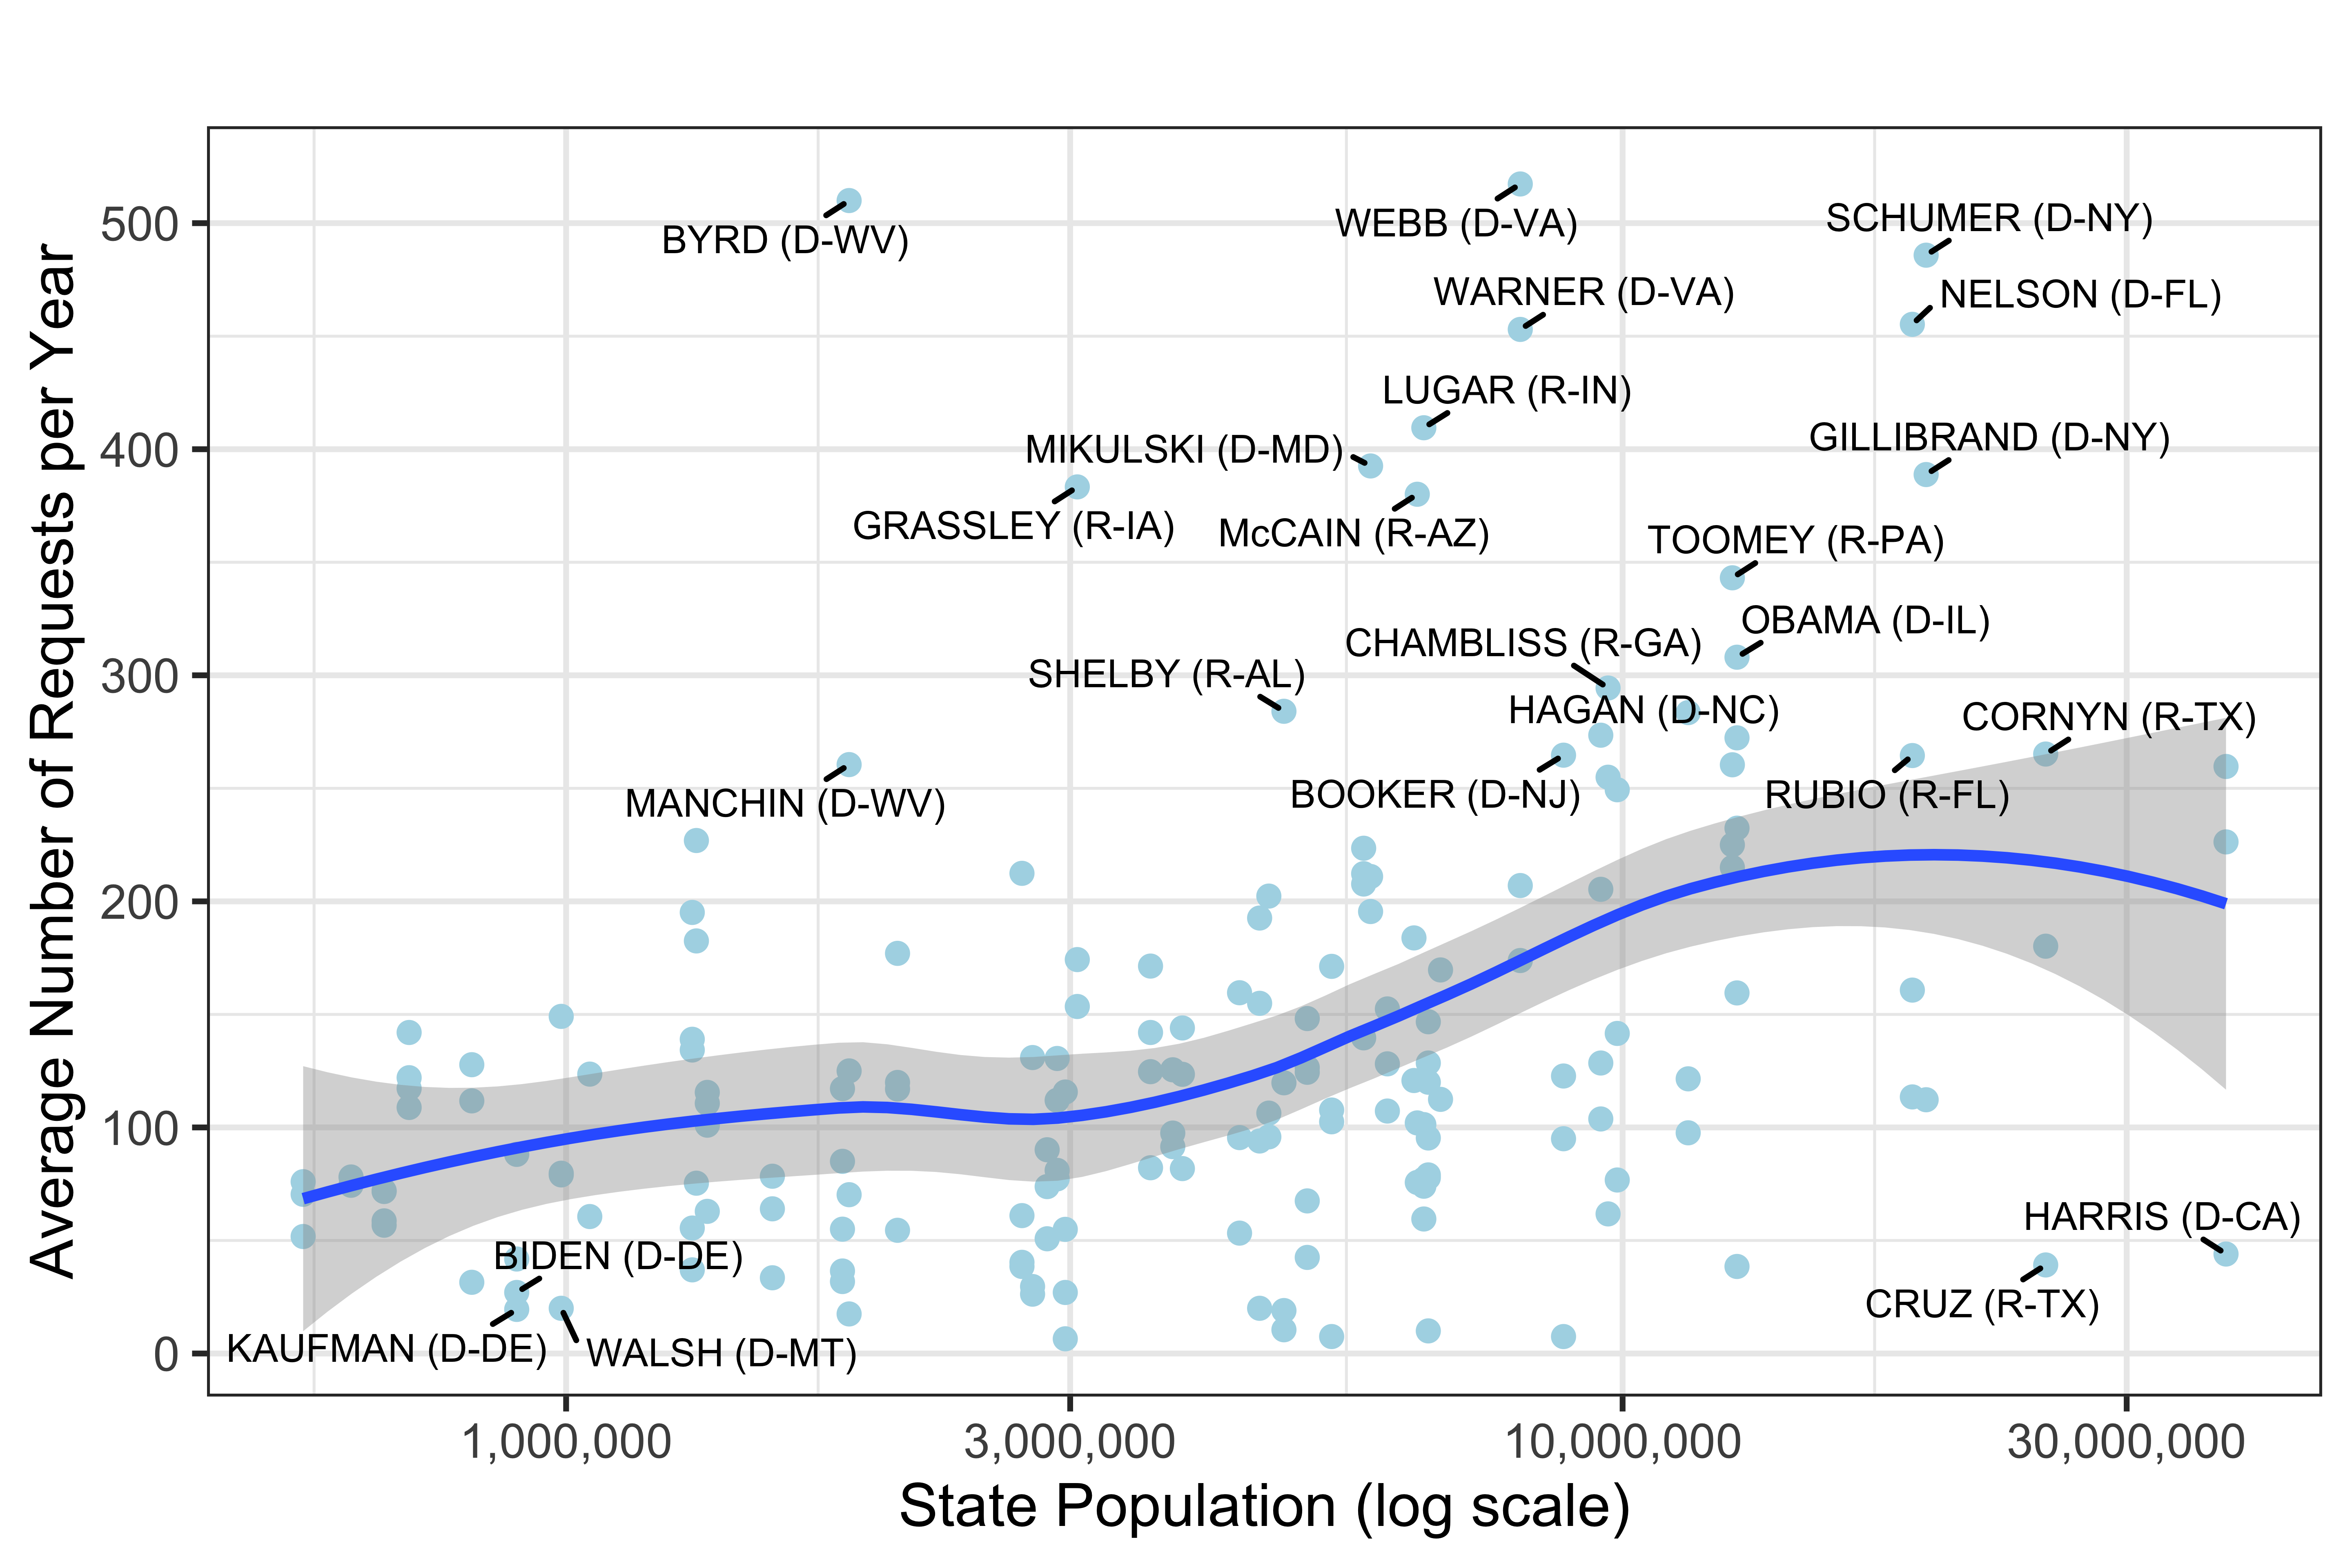
\includegraphics{figs/pop-1}}
\end{figure}

We expect the number of times a legislator contacts a particular agency to correlate with their districts' demographic composition. To assess the correlation between demographic characteristics and the rates legislators contact agencies, we focus on two example agencies: the Veterans Administration (VA) and the Social Security Administration (SSA). We measured the prevalence of two groups in the district: veterans---the residents who might plausibly need assistance navigating the VA---and residents who are over 65 years of age---and therefore satisfy the age eligibility for social security. We then run a simple bivariate regression of the total number of contacts a legislator made to each agency on the proportion of constituents who are veterans or who are over 65.  
In both instances, we find a correlation between district composition and the number of times legislators contact the agency. 

%% MOVE THIS TO APPENDIX AND ADD REGRESSION TABLE
%For example, for the VA, we find that a one percentage point increase in the proportion of residents who are veterans is associated with an increase of about .84 constituency service requests to the agency. Similarly, a one percentage point increase in the proportion of residents over 65 is associated with an increase of an additional 0.03 requests made to the agency. Overall, this suggests that legislators' efforts are correlated with the district's demographic composition.  

%% MORE NEEDED HERE

\subsection{Do Voters Demand More of More Powerful Legislators?}

Can variation in demand for constituency service explain why more experience and prestigious committee positions provide more constituency service? 

We limited the influence in demand when assessing how power and experience affect levels of constituency service above. For example, our empirical strategies in Sections \ref{s:prestige}, \ref{s:tenure}, and \ref{s:priority} account for static demand based on characteristics of the district. Districts composed of veterans might see more demand for assistance with the Veterans' Administration, or districts with older residents might have greater demand with the social security administration. Because our analyses include either legislator-agency or district fixed effects, we compare how the levels of constituency service change holding constant demand related to fixed district characteristics. Furthermore, theories of legislator capacity suggest that legislators use their increased capacity and resources to solicit constituency service requests and thus generate demand. Constituent demand driven by shifts in behavior is indeed a necessary part of the increased constituency service we attribute to increased capacity and resources in Sections \ref{s:prestige}.

Yet, we might expect that a legislator's experience or power in Congress could affect constituency demand, even without legislators using their increased capacity and resources to generate demand, as implied by theories focusing on legislator capacity. Constituents could, for example, direct more of their demands to legislators who are more powerful or who have been in Congress for longer because they don't know or trust new representatives (holding constant legislators' levels of soliciting constituency service requests). In this section, we investigate whether that additional constituent demand could plausibly explain our results. We find limited effects of legislator tenure on demand for constituency service using two distinct approaches. 

First, building on the theoretical discussion in Section \ref{s:theory}, we might worry that legislators' increasing prestige leads them to have higher name recognition, causing constituents to direct their demands to them. % TODO: NULL EFFECT? MAKE THIS DISCUSSION ACCURATE:
%We show, however, that as legislators acquire more institutional power in Congress, it does not cause an increase in name recognition. 
While more experienced legislators do have higher name recognition, name recognition increases do not align with the increases in constituency service that legislators provide their constituents, making name recognition a poor explanation for the increased level of constituency service.  

Second, if constituents direct their demands to more experienced or powerful legislators, we should observe spillover across legislators. When new members are elected, constituents should redirect their demands for service to more experienced legislators who are better known to the constituent seeking help. We find no such increase in the level of constituency service provided by more experienced legislators. When a new legislator replaces an incumbent, other members of Congress and same-state senators do not increase in their level of constituency service. This lack of spillover from new to experienced representatives suggests that constituents are not merely directing demands to more experienced legislators. Instead, members of Congress can both solicit and fulfill constituency service demand when they have more experience and capacity (e.g., an organized office and resources that come with committee appointments). As their capacity expands, they able to solicit and provide more constituency service.  %TODO Find a place to discuss how legislators create demand as they gain capacity; this is a strong point, but we only touch on it briefly.

\subsection{The Limited Effects of Prestige and Tenure on Name Recognition}
To assess how increased power and time in Congress affects legislator's name recognition, we use the Cooperative Congressional Election Study (CCES) cumulative file. CCES collects a set of survey responses from 2006-2018, providing 452,755 individual-level responses. All respondents were asked if they approve of their representative in the US House and both senators. If the respondent provided an assessment of the elected official, we coded the respondent as recognizing the legislator's name. If the respondent selected the option that they had never heard of the representative or were not sure, then we code them as not recognizing the legislator.

We estimate the average name recognition for each legislator in each survey $Y_{it}$, or the proportion of respondents who provide an evaluation of the legislator. We then use difference-in-differences regressions to assess how legislators' name recognition changes as they spend more time in Congress.  

%TODO NEW TABLE WITH ONLY DIFF-IN-DIFF
\begin{table}[hbt!]
\caption{Limited Changes in Name Recognition} \label{t:namerec1}

\begin{minipage}{\textwidth}
\begin{center}
\begin{tabular}{l*{2}{c}}
\toprule
                    &\multicolumn{1}{c}{(1)}&\multicolumn{1}{c}{(2)}\\
\midrule
Second Year         &     -0.0385&     -0.0230\\
                    &   (0.00642)&   (0.00641)\\
Fourth Year         &     -0.0263&    0.000275\\
                    &   (0.00646)&   (0.00682)\\
Sixth Year          &     -0.0281&     -0.0112\\
                    &   (0.00676)&   (0.00634)\\
Eighth Year         &     -0.0132&     0.00132\\
                    &   (0.00663)&   (0.00674)\\
\midrule
Legislator Fixed Effects&            &  \checkmark\\
Year Fixed Effects  &            &  \checkmark\\
Observations        &        3667&        3667\\
\bottomrule
\multicolumn{3}{l}{\footnotesize Robust standard errors in parentheses, clustered at legislator level}\\
\end{tabular}

\end{center}
\end{minipage}
\end{table}

%TODO MOVE TO APPENDIX?
%In the paper, we presented that the results of a difference-in-difference model that showed no relationship between time in office and name recognition. Here 
First, we discuss the cross-sectional version of this model, which shows an increase in name recognition but is severely confounded because name recognition likely leads to reelection and more time in office. Additionally, changes in name recognition do not follow the same pattern as changes in constituency service. Whereas changes in constituency service even after the first two years in office, name recognition continues to increase. If name recognition were driving our results, we would expect to see constituency service increase in legislators' fourth, sixth, and eighth years; none of which we saw in Table \ref{t:prestige1}. (Recall that across specifications in Table \ref{t:prestige1}, levels of constituency service provided were stable after year 2, controlling for legislator and district characteristics.)

The effects of time in office on name recognition do not align with observed shifts in constituency service from Table \ref{t:prestige1}.
The first column of Table \ref{t:namerec1} shows average name recognition of legislators' tenure in the House and Senate. Legislators who are newer to Congress have lower-levels of name recognition than other legislators who have been in Congress for longer. Further, we continue to see lower-levels of name recognition for legislators at the end of their second year, then for legislators serving in their 10th year and beyond. Both the persistence of this difference and the rate at which it changes suggest that name recognition is a poor explanation for why legislators provide more constituency service after their first year. Even second-year legislators---when the decrease in constituency service has already begun to attenuate---continue to have lower name recognition.  % SECOND-YEAR LEGISLATORS TELLS US NOTHING ABOUT CHANGE IN YEAR 1; IT COULD BE GREATER AND THUS CONSISTANT WITH DEMAND DRIVER

Within-legislator variation in name recognition does not appear to explain shifts in levels of constituency service that we observe. % MORE ON DIFF-IN_DIFF IF WE ARE KEEPING THIS SECTION

%TODO IF WE KEEP THIS SECTION: THERE ARE NO COLUMNS 3-6 WITH CHAIR TREATMENTS IN THE TABLE. COMMENTING OUT FOR NOW
% The third column of Table \ref{t:namerec1} shows that, on average, legislators who hold more power in Washington do have higher name recognition back in the district. Yet, using a difference-in-differences design to make within-legislator comparisons over their careers, we see that these differences disappear. Column 4 shows that when legislators acquire more power in Washington, it has little effect on their name recognition with constituents. And finally, columns 5 and 6, which include both tenure controls and prestige, show the same basic pattern: increasing time in Washington does little to affect name recognition back in the district.  


\subsection{No Evidence that Demand for Constituency Service Shifts Toward More Experienced Legislators}
This section presents a more direct test of whether constituent demand explains variation in the level of constituency service that legislators provide. If constituents shift demand to more experienced legislators, and such a shift could explain levels of constituency service, then we should observe such shifts when a new member is elected.  Suppose constituents merely redirect demand for constituent service in response to legislators' experience. In that case, the level of constituency service that incumbent legislators provide should increase when new representatives replace other incumbents from their state.  Suppose constituents shift demand based on legislator experience (as required for shifts in demand to explain our results). In that case, they should redirect their demands away from newly elected legislators towards other representatives. The most natural target for the constituent demands would be one of the senators representing the constituent's state. A more experienced House member may also receive more demands for constituency service.

To assess whether constituents redirect demand towards other more experienced legislators when new members replace their more experienced incumbent representative, we examine how experienced legislators' levels of constituency service change in response to having new representatives in their state. We measure new members in the state in two ways: either the proportion of House members and senators in the state who are new or an indicator for whether there is a new House member or senator in the state. As in Section \ref{s:prestigeresults}, we measure the number of requests made by a district's representative in a particular year. Using this dependent variable, we estimate a series of difference-in-differences regression where the treatment is new members in the state. We include district and year fixed effects. Further, we restrict the regression to incumbent legislators only.   

Table \ref{t:spill1} presents the estimates of this regression. The first two columns are estimated on all incumbent legislators. They show that neither the proportion of new members nor a new member significantly affects the level of constituency service that other legislators in the state provide. Columns 3 and 4 of Table \ref{t:spill1} reveal the same pattern when focusing on senators only. The estimated effects of new legislators do not approach statistical significance.  

   

\begin{table}[hbt!]
\caption{Little Evidence of Spillovers from New Legislators} \label{t:spill1}

\begin{minipage}{\textwidth}
\begin{center}
\begin{tabular}{l*{4}{c}}
\toprule
                    &\multicolumn{1}{c}{(1)}&\multicolumn{1}{c}{(2)}&\multicolumn{1}{c}{(3)}&\multicolumn{1}{c}{(4)}\\
\midrule
Proportion New Legislators&       5.143&            &      -1.494&            \\
                    &     (8.089)&            &     (20.06)&            \\
At Least One New Legislator&            &       1.625&            &       3.847\\
                    &            &     (2.031)&            &     (4.812)\\
\midrule
District Fixed Effects&  \checkmark&  \checkmark&  \checkmark&  \checkmark\\
Year Fixed Effects  &  \checkmark&  \checkmark&  \checkmark&  \checkmark\\
Senators Only       &            &            &  \checkmark&  \checkmark\\
Observations        &        6080&        6080&        1182&        1182\\
\bottomrule
\multicolumn{5}{l}{\footnotesize Robust standard errors in parentheses, clustered at district level}\\
\end{tabular}

\end{center}
\end{minipage}
\end{table}


\section{Conclusion} \label{s:conclude}
% SUMMARY 
Using a new data set on legislators' requests made to federal agencies, we show that as legislators gain experience and power, they both gain capacity and shift priorities toward policy work. We also show that legislators make fewer service requests at the start of their career and that new legislators make substantially fewer service requests than their more experienced colleagues. We also show that the institutional power gained through prestigious committee appointments, especially committee chairs, increases legislators' capacity and that they use this capacity to provide more constituency service and do more policy work.

%Theories asserting that capacity matters correctly predict that the levels of both constituency service and policy work increase as legislators gain experience and institutional power in Congress.
%Theories asserting that legislators shift priorities correctly predict that the ratio of policy work to constituency service increases as legislators spend more time and gain institutional power in Congress.
%Empirically, the net result of both effects is a net increase in the levels of both policy work and constituency service as legislators spend more time and gain institutional power in Congress; there is no tradeoff.

% FORMAL MODELS 
Our results are broadly consistent with the predictions about constituency service provision from multi-task selection models, such as \cite{AshworthBuenodeMesquita2006}. Constituent service helps explain incumbency advantage in these models because it provides legislators the opportunity to demonstrate their ability to their constituents. Our results show that legislators take advantage of this opportunity, particularly as they become more powerful. With greater capacity, experienced and powerful legislators have an advantage in providing service over new representatives. Constituency service thus advantages incumbents because switching to a new representative implies a decline in particularistic services to the district. 

% PRACTICAL IMPACT: NOT A CONCLUDING PARAGRAPH 
The findings from this paper also flip some of the concerns motivating proposed institutional reforms on their heads. For example, advocates of term limits often argue that elected officials lose touch with their district. In contrast, we show that the more experienced legislators provide more attention to their district, even as they take on more policy work.  

%Future research should examine mechanisms of increasing capacity. This could include explicit measures of office organization and capacity and more nuanced measures of institutional power. This could also include measuring agency responsiveness to legislator requests. Likewise, future research could examine mechanisms related to shifting priorities. Finally, future work could include legislators substantive areas of expertise. Does expertise increase a legislators capacity to act in certain area (e.g. certain agencies), leading to more capacity to do constituency service? Does increased institutional power lead legislators to develop expertise, for example in certain committee work or specialized policy work that builds their capacity to influence certain agencies? 

Taken together, our findings show that the reelection motivation remains a potent force for even the most powerful legislators in Washington.  Rather than use increased power in the institution as an excuse to be less attentive to the district or increased time in Washington to be less interested in their constituencies, our results show that legislators with more power and experience provide more service to their district.  Even if legislators catch ``Potomac Fever" they still remember their job as constituent ombudsman. 

%TODO BETTER CONCLUSION
%Rather than forgetting about the district and contracting Potomac Fever, it would appear that more experience and power in Congress enables legislators to deliver particularistic goods to the district more effectively.  

\singlespacing

\bibliography{congress2019}

%\newpage
%\listoftodos[Notes]

\clearpage
\appendix
\setcounter{table}{0}
\renewcommand{\thetable}{A\arabic{table}}

\section*{Appendix}

%%% Ellie: I manually changed the input code here so that the entire table would fit here.  
\input{../tables/FOIA_response.tex}


\section{Contact Codebook} \label{a:codebook}
\singlespacing
%%% Note: From Ellie. I deleted everything here that we're not using in this paper.  

We provide the following codebook to a team of hand-coders to code each case of Congressional contact with federal agencies and extract information about the legislator. The codebook provides a series of steps to move from raw correspondence logs to data formatted for our analysis.  

\subsection{Congressional Correspondence Log Coding Guidelines}

The first step is to identify the columns that contain the member of Congress (or Committee), the date that the member-initiated correspondence, and the column that best describes the subject. These should be named FROM, DATE, and SUBJECT. 

We aim to classify the subject of correspondence between members of Congress and government agencies. You can do this using keywords (potential keywords in italics below) but may also require googling subject lines (e.g., what does this acronym mean in this context!?) and inferring why the legislator made the request. Doing so may require identifying a member's relevant policy positions. For example, if the subject is "mining regulations" or "open internet," a member's voting history on related bills or donations from the industry may help us infer if the letter was policy work on behalf of the industry (type 4) or not (type 5). Limiting your search to a date range around the letter date may yield relevant public statements. If you have questions, find something interesting, or, in your efforts to classify a confusing correspondence, you discover information like a related public statement, note it in the NOTES column. In some cases, columns other than the SUBJECT may offer helpful information. This may be difficult at first but will get easier. \\

The outcome is a spreadsheet with the first columns being FROM, DATE, SUBJECT, TYPE, CERTAINTY, ALT\_TYPE.\\


Below are five potential codes for the TYPE and three potential codes for your level of CERTAINTY that it is this type. If you are less than Very Certain (i.e., if only Fairly Certain, or Toss Up), also record your second best guess as ALT\_TYPE, otherwise leave this column blank. Only leave NOTES if you think it would be helpful for the team to revisit the entry.

\subsubsection{TYPE}

1 = Personal Service\\

\hfill\begin{minipage}{\dimexpr\textwidth-2cm}
Definition: Individual, non-commercial constituent service.\\
Examples: Help with a government form, passport, visa, back pay, military honor, enlistment, criminal case, request for personal information (e.g., one’s FBI file), disability application, worker compensation, personal complaint, discrimination case, job application, health insurance, financial services complaints, etc.\\
\end{minipage}

2 = Commercial Service - Transactional \\

\hfill\begin{minipage}{\dimexpr\textwidth-2cm}
Definition: Anything related to a specific individual case by a business (including business owners like farmers and consultants).\\ 
General Examples: Help with a grant application, payment, loan, or contract (buying anything from or selling anything to a government agency). Help with an individual case of tax assessment, fine, or regulatory enforcement action. Help with public relations on behalf of a business.\\
Specific Examples: allocation of radio spectrum, a case against a company, tax dispute, contract for the purchase of military surplus, crop insurance distribution, debt settlement, foreclosure assistance, a fine for a law violation, etc. \\
\end{minipage}

3 = Government and Nonprofit Service - Transactional\\

\hfill\begin{minipage}{\dimexpr\textwidth-2cm}
Definition: Same as for (2-Commercial Service), but for municipal or state governments (including cities, counties, etc.) or non-business-oriented nonprofit organizations (i.e., NOT ones that represent an industry or trade association) \\
\end{minipage}

4 = Commercial Service - Policy \\

\hfill\begin{minipage}{\dimexpr\textwidth-2cm}
Definition: Anything applying to a class of commercial activity or businesses (e.g., shipping, airlines, agriculture), including legislation, bills, acts, appropriations, authorizations, etc. \\
General Examples: Authorization of or appropriation to a government program targeted towards a particular industry or industries. Regulation of industry or commercial practice or competition.\\
Specific Examples: Milk prices, insurance or loan eligibility criteria, purchasing policies, crop insurance rates, pollution criteria, classification of products for trade or taxation, conservation appropriation, worker visa types, restrictions, or caps, etc.\\
\end{minipage}
 
5 = Policy Work - NOT in the service of any individual, business, specific industry.\\

\hfill\begin{minipage}{\dimexpr\textwidth-2cm}
Examples of Policy Work: 
 \begin{tight_itemize} 
 \item Lawmaking 
\item Request for policy-relevant information. This includes prospective legislation, legislation under consideration, or already implemented legislation that requires oversight.  
\item Oversight
\item Committee requesting a report or testimony at a hearing
\item Requesting clarity on an agency rule
\item Lobbying administrative policy
\item Agency rulemaking with non-commercial implications (comments on agency rulemaking may often be (3)) 
\item Political work
\item Meeting with organized constituent groups (e.g. workers, people with disabilities, environmentalists) about policy (meetings with industry groups generally fall under (4)).
\item Media requests
 \end{tight_itemize} 
\end{minipage}
\bigskip


6 = Other \\

\hfill\begin{minipage}{\dimexpr\textwidth-2cm}
	Suggest a new category in the NOTES column, only if you cannot fit it under 1-4. For example, requesting dirt on one's political opponents could be called "partisan" as none of the above. Other specific types: thank you (for thank you notes with no other information), congratulations (for congratulatory correspondence on appointments or retirements with no other information), family member (for correspondence on behalf of a family member) \\
\end{minipage}


\end{document}






 



 